\documentclass[10pt,letterpaper,]{book}

\usepackage[activeacute, spanish]{babel}
\spanishdecimal{.} % usar puntos en vez de comas en modo matematico
\usepackage[utf8]{inputenc}
\newtheorem{definicion}{{\b Definici\'on}}[section]

% ------------------------- ini-imeta.tex -------------------------
 \usepackage[colorlinks=true,urlcolor=blue]{hyperref} %requerido para \hypersetup
\newcommand{\titulo}{Estructura de datos.}
\newcommand{\autor}{Wilson S. Tub\'in}
\newcommand{\tema}{EDD}
\newcommand{\blog}{https://wilsoneliseo.wordpress.com/}
\newcommand{\institucion}{Wilson Eliseo GT}
\newcommand{\departamento}{Ingeniería}
\newcommand{\firma}{WeGT}
\newcommand{\correo}{wilsoneliseogt@gmail.com}

\hypersetup{
  pdftitle={\titulo},
  pdfauthor={\autor},
  pdfsubject={\tema},
  pdfcreator={\blog},
  pdfproducer={\institucion},
  pdfkeywords={\firma}
}
% ------------------------- fin-imeta.tex -------------------------

\usepackage{amsmath} % matematica
\usepackage{amsfonts}
\usepackage{amssymb}

%-------------------------------------------------------------------------------
%	PERSONALIZACION ENCABEZADO Y PIE DE PAGINA
%-------------------------------------------------------------------------------
\usepackage{fancyhdr} % requerido para personalizar encabezado y pies de pagina
\usepackage{lastpage} % requerido para personalizar pies de pagina
\pagestyle{fancy} % todas las paginas tienen encabezados y pies
\fancyhead{} % encabezado predeterminado en blanco
\fancyfoot{} % pie de pagina predeterminado en blanco
\fancyhead[C]{\titulo $\, \bullet$ \tema $\, \bullet$ \href{\blog}{\autor} } 
\rfoot{P\'agina\ \thepage\ de\ \protect\pageref{LastPage}} % pie derecho


%-------------------------ini-icodigo.tex-------------------------

% PAQUETES REQUERIDOS----------------------------------------|
\usepackage{listings} % requerido para insercion de codigo
\usepackage{courier}
\usepackage{color} % requerido para personalizacion de colores


% CONFIGURACION DEL CODIGO DE INCLUSION----------------------|
\definecolor{gray97}{gray}{.97}
\definecolor{gray75}{gray}{.75}
\definecolor{gray45}{gray}{.45}
\definecolor{morado}{RGB}{116,6,164}

\lstset
{
  frame=Ltb,                    % marco
  framerule=0pt,                % borde del marco
  aboveskip=0.5cm,
  framextopmargin=3pt,
  framexbottommargin=3pt,
  framexleftmargin=0.4cm,
  framesep=0pt,
  rulesep=.4pt,
  backgroundcolor=\color{gray97}, %fondo del frame
  rulesepcolor=\color{black},
  texcl=true,
  %
  stringstyle=\color{morado},   % cadenas de color purpura
  showstringspaces=false,       % mostrar marca en los espacios
  basicstyle=\small\ttfamily,   % estilo basico de caracteres
  commentstyle=\usefont{T1}{pcr}{m}{sl}\color{gray45}\small, % comentarios small
                                                     %dark green, fuente courier 
  keywordstyle=[1]\color{blue}\bf, % funciones en negrita y azul
  keywordstyle=[2]\color{purple},  % argumento de funciones en purpura
  keywordstyle=[3]\color{blue}\underbar, % funciones subrayadas y azules
  identifierstyle=,             % nada especial a identificadores
  %
  numbers=left,
  numbersep=15pt,
  numberstyle=\tiny\color{gray45}, %estilo de numeracion
  numberfirstline = false,
  breaklines=true,              % quebrar lineas largas
  stepnumber=1,                 % numerar cada linea
  tabsize=2,                    % dos espacios por cada tab
}


\lstdefinestyle{miEstilo}
{
  language=[ansi]c++, % sintaxis para c++
  %language=[latex]tex, % sintaxis de latex
}

%-------------------------fin-icodigo.tex-------------------------


\usepackage{graphicx} % Requerido para insertar imagenes
\graphicspath{ {imgArreglos/}{imgArboles/}{imgTablasDeDispersion/}{imgTextos/}{imgExams/} }
\usepackage{float}

\usepackage{alltt}
\usepackage{color}

\usepackage[sc]{mathpazo} % Usar fuente Palatino
\usepackage[T1]{fontenc} % Usar codigicacion 8-bit
\linespread{1.05} % Espacio de linea - Palatino necesita mas espacio entre lineas
\usepackage{microtype} % Ajustar ligeramente el espaciado de letra
                       % para la estética

\usepackage{makeidx}


\author{\autor \\ \correo}
\title{\titulo}
\date{}


\begin{document}


\maketitle
\thispagestyle{empty}

\frontmatter
\chapter{Introducción}
El documento contiene algo de algoritmia, arreglos, arboles, tablas de
dispersión y textos. Todos temas vistos en el curso de estructuras de
datos de la carrera de Ingeniería En Ciencias Y Sistemas de la
Universidad De San Carlos De Guatemala.

\begin{description}
\item[Algoritmia: ] Estudio de los algoritmos
\item[Arreglos: ] Estudio de representaciones y algoritmos de manejo
  de arreglos
\item[Árboles: ] Conceptos generales y representaciones de árboles
\item[Tablas de dispersión: ] En esta unidad revisaremos otra
  estructura para uso de contenedores, que busca obtener el
  rendimiento de los arreglos lexicográficos y la flexibilidad en el
  uso de memoria de los árboles.
\item[Textos: ] Estudio de las diferentes representaciones y
  aplicaciones del manejo de textos o strings.
\item[Ejercicios de examen: ] Alguno ejercicios resueltos de
  exámen. Otros solo se presentan, más carecen de solución.
\end{description}

\let\cleardoublepage\clearpage

\mainmatter
\chapter{Algoritmia}
\label{cha:algoritmia}
Estudio de los algoritmos
\section{Eficiencia de algoritmos}

\subsection{Necesidad de la algoritmia}
\label{sec:necesidad-de-la}

Dado un problema cualquiera que se desee implementar, habran casi
tantas soluciones efectivas, como programadores trabajen en ella.  Sin
embargo sólo habrá una solución, que sea la más eficiente. Ésto se
debe a que parte de la programación involucra arte y creatividad, y
cada persona piensa de manera diferente.

Dado que siempre estamos interesados en reutilizar lo existente, si
buscamos una solución para un problema, seguramente encontraremos
varias implementaciones, y deberemos elegir una de ellas como la más
eficiente para utilizar.

Para ésto, primero tenemos tener claro la diferencia entre efectivo y
eficiente:

\begin{description}
\item[Efectividad: ] Capacidad de lograr el efecto que se desea o se
  espera.
\item[Eficiencia: ] Capacidad para lograr un fin, empleando los medios
  más adecuados
\end{description}

Claro, definir <<los medios más adecuados>> depende de la solución y lo
que se declare importante.  Por ejemplo: si se desea ir el país vecino
¿cuál es el medio más adecuado para llegar? ¿por bus, por avión,
caminando? Tomar la decisión del medio, dependerá de qué el lo
importante que se desee lograr. Si tenemos tiempo y nos gusta
disfrutar el paisaje, el mejor medio es el bus, si tenemos un negocio
importante que nos perderíamos si no llegaramos a tiempo, el medio
adecuado sería el avión.

\subsection{Eficiencia de algoritmos}
\label{sec:efic-de-algor}

Para lograr comparar dos algoritmos tenemos dos opciones:
\begin{description}
\item[Método empírico (a posteriori): ] Consiste en realizar las dos
  implementaciones y realizar ejecuciones similares, en la misma
  máquina y con la misma cantidad de datos, y comparar los tiempos de
  ejecución. Este método es la medida más exacta que se puede lograr,
  pero tiene la desventaja es que no siempre hay tiempo para hacer
  varias implementaciones o, si ya están hechas, hacer ambas
  implementaciones puede ser compleja y no ser factible.
\item[Método teórico (a priori): ] Consiste en realizar un análisis
  matemático de los algoritmos y determinar una medida de la
  eficiencia. Ésto tiene la ventaja que no necesita una implementación
  real de los algoritmos, ya que basta con un esbozo de la
  implementación para realizar el análisis.
\end{description}

En el caso de los algoritmos, los medios para lograr la eficiencia se
refieren a la utilización de tiempo y memoria, los cuales se tienen
que equilibrar, y nos referimos a ellos en el estudio de
\textbf{complejidad espacial} (eficiencia en el uso de la memoria) y
\textbf{complejidad temporal} (eficiencia en el tiempo de ejecución).

La \textbf{complejidad espacial} se refiere a cuánta memoria necesita
un algoritmo para ejecutarse completamente.  Aunque actualmente se
tiene la impresión que no es tan determinante para la construcción de
un algoritmo como solía ser, sigue siendo un factor a tomar en cuenta
al momento de implementar una solución, principalmente en ambientes
concurrentes, como soluciones web, o en ambientes más restringidos
como las soluciones móviles.  En el ambiente web, un servicio
relativamente simple, si tiene alta complejidad espacial (usa mucha
memoria), al atender a miles de clientes, puede colapsar cualquier
servidor.  En un ambiente móvil, la memoria es más limitada que en una
PC o servidor, por lo que se debe tener presente la cantidad de
memoria a utilizar.

Anteriormente, era crítico el análisis de complejidad espacial, ya que
si un programa no cabía en memoria (programa más datos) no era posible
ejecutarlo.  Actualmente, ésto ya no es restricción debido al uso de
la memoria virtual, pero ya que ésta involucra la utilización de disco
duro, igualmente se debe vigilar el uso de la memoria para no degradar
el rendimiento del sistema.  Simplificando a niveles prácticos el
análisis de la complejidad espacial, básicamente podemos decir que se
trata de determinar el tamaño del ejecutable, adicionado a cuánta
memoria necesita cada elemento de una estructura, multiplicado por el
máximo número de elementos, y ésto lo comparamos con la memoria
disponible.

\begin{quote}
   \textbf{memoria libre <= tamaño\_ejecutable + tamaño\_elemento * máximo\_elementos}
\end{quote}

En cada estructura que estudiemos, haremos esta comparación, como un
hábito que debe tener cada programador.

En el caso de la \textbf{complejidad temporal}, sí se requiere un
análisis más detenido para llegar a una conclusión ¿cómo podemos
analizar teóricamente el tiempo de ejecución sin ejecutar el
algoritmo? ¿en qué computadora se realizará? dado que diferentes
computadoras utilizan diferentes velocidades de ejecución ¿qué unidad
de tiempo utilizar?  ¿milisegundo o nanosegundos?

Para realizar el análisis de un algoritmo, independientemente de la
computadora a usar, vamos a utilizar el siguiente principio:

\begin{description}
\item[Principio de la invarianza: ] Si dos implementaciones tardan
  respectivamente $T_1(n)$ y $T_2(n)$, entonces para resolver un problema
  con datos de tamaño $n$, existirá siempre una constante positiva $c$ tal
  que $T_1(n) \leq c * T_2(n)$ para un $n$ suficientemente grande
\end{description}

Ésto significa que $T_2(n)$ será $c$ veces más rápido que $T_1(n)$, sin
importar la computadora.  Si en una máquina $T_1(n)= 5$ segundos y $T_2(n)=
1$ segundo, en otra máquina más rápida $T_1(n)= 5 ms$ y $T_2(n)= 1 ms$.  En
otras palabras $T_2(n)$ siempre más rápido que $T_1(n)$, en cualquier
máquina.

Por lo tanto no necesitamos una unidad de tiempo específica para
comparación, ya que nuestro análisis es independiente de la máquina.
Usaremos una unidad de tiempo adimensional que denominaremos
\textbf{tiempo mínimo} denotado por \textbf{t} que es el tiempo en el
que cualquier procesador ejecuta la instrucción más simple, como una
asignación o expresión matemática.

Adicionalmente, la unidad de tiempo es irrelevante ya que la medida de
eficiencia no es un número, sino una función:

\begin{definicion}
  \textbf{Función de orden O(n)}.  Se dice que \textbf{f(n)} es de
  orden \textbf{g(n)} si y sólo si
  \[ f(n) \leq c * g(n)  \;\;\; para\; todo\; n \geq n_0 \]
\end{definicion}

donde $c$ y $n_0$ son constantes positivas independientes de $n$

\begin{itemize}
\item[Ejemplo 1. ]  sea $f(n) = 3n^3 + 2n^2 $.  ¿Podemos decir que
  $O(f(n) ) = n^3$ ?  si tenemos $c = 5$ y $n_0 = 0$\\

se cumple que
\[f(n) \leq 5 * g(n) \;\;\;para\; todo\; n \geq 0\]
\begin{eqnarray*}
  3n^3 + 2n^2  & \leq & 5n^3\\
 3n^3 + 2n^2  & \leq & 3n^3 + 2n^3\\
2n^2  & \leq & 2n^3\\
n^2  & \leq & n^3
\end{eqnarray*}
para todo $n \geq 0$
\item [Ejemplo 2. ]  sea $f(n) = 3n+ 1$.  ¿Podemos decir que $O(f(n) )
  = g(n) = n$ ? si tenemos $c = 4$ y $n_0 = 1$ \\

se cumple que
\[f(n) \leq 4*g(n) \;\;\;para \; todo \;n\; \geq 1\]
\begin{eqnarray*}
  3n+ 1 & \leq & 4n \\
  3n+ 1 & \leq & 3n + n \\
  1 & \leq & n
\end{eqnarray*}
 para todo $n \geq 1$
\end{itemize}

En nuestros análisis no podremos hacer una hipótesis y comprobarla,
como en los ejemplo anteriores, sino que dada la función f(n),
deberemos deducir g(n).  Ésto podremos hacerlo usando las siguientes
propiedades de la función O(n), cuya deducción está fuera del alcance
del curso:

\subsubsection{ Propiedades de O(n)}
\label{sec:propiedades-de-on}

\begin{itemize}
\item las constantes no importan: O[ c * f(n) ] = c * O[ f(n) ] = O[
  f(n) ]
\item Regla de la suma:
  \begin{itemize}
  \item O[ f(n) + t(n) ] = max [ O( f(n) ), O( t(n) ) ]
  \item O[f(n)] + O[t(n)] = O [f(n) + t(n)]
  \end{itemize}
\item regla de la multiplicación: O[f(n)] * O[t(n)] = O[f(n) * t(n)]
\item anidación: O [ O(f(n)) ] = O [f(n)]
\end{itemize}

De los ejemplos anteriores podemos deducir O(n), aplicando estas
propiedades así:

\[
\begin{array}{lll}
  O(3n^3 + 2n^2 )&&\\
  & Regla \;de\; la\; suma:& O(3n^3+2n^2)=max(O(3n^3),O(2n^2))=O(3n^3)\\
  &  Regla \;de\; las\; constantes:&O(3n^3)=O(n^3)=n^3\\
  O(3n+1)&&\\
  &Regla\; de\; la\; suma:&O(3n+1)=max(O(3n),O(1))= O(3n)\\
  &Regla\; de\; las\; constantes:&O(3n)=O(n)=n 
\end{array}
\]

En general, lo resultados de O(n) se pueden clasificar en los
siguiente órdenes (del mejor al peor):

\begin{itemize}
\item constante:   $O(f(n)) = c$, donde $c$ es una constante
\item lineal:          $O(f(n)) = n$
\item logarítmica: $O(f(n)) =  log_c(n)$
\item progresiva, geométrica o polinomial: $O(f(n))=n^c$ , $c>=2$.
  Incluye cuadrático ($n^2$) y cúbico ($n^3$)
\item Exponencial:  $O(f(n)) = c^n$, para $c > 1$
\end{itemize}

Los dos últimos órdenes son especialmente deficientes, y en cualquier
lado que los encontremos, debemos esforzarnos en mejorar el
rendimiento.

\section{Eficiencia de algoritmos no recursivos}
\label{sec:efic-de-algor-1}
Para determinar la eficiencia de un algoritmo debemos realizar los
siguientes pasos:

\begin{enumerate}
\item Determinar una función del tiempo de ejecución del algoritmo
  para \textbf{n} datos: T (algoritmo(n) ) = T(n)
\item Aplicar las propiedades de O(n) para deducir O(T(n))
\end{enumerate}

Dado el software es matemática, tal como demostró Allan Turing,
entonces todo algoritmo tiene una expresión matemática y viceversa, es
posible hacer una expresión matemática, T(n), de cualquier algoritmo .

Para ésto utilizaremos los principios del teorema de la programación
estructurada, la cual establece que todo algoritmo puede ser realizado
utilizando sólo las siguientes instrucciones básicas:

\begin{itemize}
\item Asignaciones y expresiones simples
\item Secuencia
\item Condición
\item Ciclos
\end{itemize}

Si podemos establer una función de tiempo para cada una de estas
sentencias, entonces podremos deducir dicha función para el algoritmo
completo.

Recordar que usamos medidas de tiempo teóricas (adimensionales) =
\textbf{t} = tiempo de la instrucción más simple o rápida de ejecutar
en el procesador

\subsection{ Asignaciones y expresiones simples}
\label{sec:asign-y-expr}

\begin{eqnarray*}
T(asignacion) &=& T(expresion \; simple) = {\bf t}\\
\mapsto O(asignacion) &=& 1 \;\;  ( orden \;constante )
\end{eqnarray*}

Ésto incluye sentencias como
\begin{eqnarray*}
  \label{eq:1}
  x& =& y ;\\
  y &=& 5 + y * z ;
\end{eqnarray*}

\subsection{Secuencia de instrucciones}
\label{sec:secu-de-instr}

\begin{eqnarray*}
  T(secuencia) &=& T (sentencia1) + T (sentencia2) + \ldots +T(sentencia \;n)\\
  \\
  \mapsto O(secuencia) &=& O[T (sentencia1) + T (sentencia2) +\ldots+ T(sentencia \;n) ]\\
  &=& Max\Bigl[\;O\bigl(T (sentencia1)\bigr),\, O\bigl(T (sentencia2)\bigr) +\ldots+ O\bigl(T(sentencia\; n)\bigr) \;\Bigr]
\end{eqnarray*}


\subsection{Instrucciones condicionales}
\label{sec:instr-cond}

\begin{verbatim}
if ( condicion ) {
    sentenciaThen
}else{
    sentenciaElse
}
\end{verbatim} 


\begin{eqnarray*}
  T(if) &=& T ( condicion ) + max \bigl[ \;T ( sentenciaThen ), \;\;T (sentenciaElse) \;\bigr]\\
  \\
  \mapsto O(if) &=& O[\; T ( condicion ) + max ( T ( sentenciaThen ), \;\;T (sentenciaElse) )\;]\\
  &=& max \Bigl[\; O\bigl(\,T ( condicion )\,\bigr), \;O\bigl(\, T ( sentenciaThen )\,\bigr), \;O\bigl(\,T (sentenciaElse)\,\bigr) \;\Bigr]
\end{eqnarray*}

\subsection{Instrucciones de iteración (for - while) }
\label{sec:instr-de-iter}


\begin{alltt}
{\bf for}
\end{alltt}

\begin{verbatim}
for (asignacionInicial ;  condicion ; asignacionFinal)
    sentenciaCiclo
}
\end{verbatim}

\begin{eqnarray*}
T( for ) &=& T (  asignacionInicial ) +   \bigl[\; T ( condicion ) + T ( sentenciaCiclo ) + T ( asignacionFinal ) \;\bigr] {\bf * v}
\end{eqnarray*}
donde \textbf{v}  es el número máximo de veces que se repite el ciclo

\begin{alltt}
{\bf while}
\end{alltt}

\begin{verbatim}
i = 0 ; //  asignacion inicial
while ( condicion ) {
    sentenciaCiclo
}
\end{verbatim}

\begin{eqnarray*}
  T( while ) &=& T ( asignacionInicial ) +   \bigl[ \;T ( condicion ) + T ( sentenciaCiclo ) \; \bigr] {\bf * v}
\end{eqnarray*}
donde \textbf{v} es el número máximo de veces que se repite el ciclo
en el peor de los casos


\begin{eqnarray*}
  \mapsto O(ciclo) &=& O \Bigl[\; T (  asignacionInicial ) +   [ \;T ( condicion ) + T ( sentenciaCiclo ) \;] {\bf * v} \;\Bigr]\\
  &=& max \Bigl[ \;O [ T (asignacionInicial )] +  O [\; \bigl( \; T ( condicion ) + T ( sentenciaCiclo ) \;\bigr) {\bf * v} \;]\;\Bigr]
\end{eqnarray*}
En estos casos, lo complicado suele ser determinar \textbf{v} en
términos de \textbf{n} ( v = f(n) )

\subsection{Llamadas a procedimientos}
\label{sec:llam-proc}

La llamada en sí misma es de tiempo constante, pero toma como tiempo
de la llamada, el tiempo de la ejecución completa

Está determinado por el cuerpo del procedimiento, dado que el paso de
parámetros es constante (igual que una asignación)

\subsection{Ejemplos}
\label{sec:ejemplos}

\begin{enumerate}
\item \verb|x = x + 1 ;|
  \begin{eqnarray*}
    T(n)  &=& t\\
    \mapsto O(asignacion) &=& O [ T(n) ] = O(1) = 1\;\;   (constante)
  \end{eqnarray*}
\item
\begin{verbatim}
for (i = 1; i <= n; i++ )
        x = x + 1 ;
\end{verbatim}
  $$T(for) =  T(asignacionInicial) + v * \bigl[ T(condicion) + T (cuerpoDelFor) + T (asignacionFinal) \bigr] $$
  En este caso
  $$ T (for) = t + n ( t + t + t) =  t + 3nt = t(3n+1)$$
  \begin{eqnarray*}
    \mapsto O \bigl[ T(for) \bigr] &=& O[\,t(3n+1)\,] \\
    &=& O(t)*O(3n+1) \\
    &=& O(1)*max\bigl[O(3n),\;O(1)\bigr] \\
    &=& O(3n) \\
    &=& O(n) = n\;\; (lineal)
  \end{eqnarray*}
\item
\begin{verbatim}
int A (int n) {
    x=1 ;
    while (x<n)
           x= 2 * x ;
    return x ;
}
\end{verbatim}
  \begin{eqnarray*}
  T(A) &=& T(asignacion) + T(while) + T(asignacion)\\
  T(A) &=& t +  \bigl[\, T(condicion) + T(cuerpoDelWhile) \,\bigr] * v + t
\end{eqnarray*}
$v$=número de veces que se ejecuta el cuerpo y condición del while.

¿cuánto es $v$ en términos de $n$\footnote{$n$ representa el numero de datos que recibe el argoritmo}?

Podemos hacer un algoritmo equivalente
\begin{verbatim}
int A1(int n) {
    x=1 ;
    v=0 ;
    while (x < n) {
        x = 2 * x ;
        v = v + 1 ;
    }
    cout << "v=" << v ;
    return x;
}
\end{verbatim}
Valores de $v$ y $x$ respecto a $n$

\begin{tabular}{c|c|c}
n & v & x \\ \hline
1 & 0 & x=1/v=0 \\
2 & 1 & x=2/v=1 \\
3 & 2 & x=4/v=2 \\
4 & 2 &  \\
5 & 3 & x=8/v=3 \\
6 & 3 &  \\
7 & 3 &  \\
8 & 3 &  \\ 
9 & 4 & x=16/v=4 \\
10 & 4 &  \\
. & . &  \\
16 & 4 &  \\
17 & 5 & x=32/v=5 \\ 
.. & .. &  \\
32 & 5 &  \\ 
33 & 6 & x=64/v=6 \\
.. & .. &  \\ 
64 & 6 &   \\ 
\end{tabular}
\\[.5cm]
Podemos deducir que existe una relación entre $v$ y $n$ así:
$$2^v \geq  n$$

por tanto
\begin{eqnarray*}
  \log_2(2^v) &\geq&\log_2(n)\\
  v&\geq&\log_2(n)
\end{eqnarray*}

la funcion del tiempo sería
\begin{eqnarray*}
  T[\,A(n)\,] &=& T(asignacion) + T(while)\\
  &=& t +  \bigl[\, T(condicion) + T(cuerpoDelWhile) \, \bigr] * \log_2(n)\\
  &=& t + \log_2(n)*(t + t )\\
  &=& t + 2t*\log_2(n)
\end{eqnarray*}

la función O(n) sería
\begin{eqnarray*}
  \mapsto O[\,A1(n)\,] &=& O[1 + 2*\log_2(n) ]\\
  &=& \log_2(n) \;\;\;    (logaritmico)
\end{eqnarray*}

\end{enumerate}

\section{ Eficiencia de algoritmos recursivos }
\label{sec:efic-de-algor-2}

Para calcular el tiempo de un algoritmo recursivo, básicamente es el
mismo procedimiento, pero tenemos que tener en cuenta los siguientes
cambios:

\begin{itemize}
\item Dado que es un algoritmo recursivo, la función de tiempo también
  será recursiva
\item Identificar la condición de salida del algoritmo, para que la
  función recursiva de tiempo, sea dual, con una parte no recursiva,
  definida por la condición de salida
\item Una vez definida la parte recursiva, se deberá expander a modo
  de resolver sin recursión, por medio de expansiones sucesivas.
\end{itemize}

\subsection{Ejemplo 1}
\label{sec:ejemplo-1}

\begin{verbatim}
int factorial (int n) {
    if ( n <= 0 )
        return 1 ;
    else
       return n * factorial (n-1) ;
}
\end{verbatim}

La condición de salida es $n \leq 0$, por lo tanto nuestra función de tiempo
será dual y recursiva así:
$$T[\,factorial(n)\,]=T(n)$$
\begin{equation*}
  \label{eq:definicion por partes}
  T(n) = \left\{
    \begin{array}{ll}
      \mathrm{si\ } n \le 0 \; :    &  T(condicion)+T(asignacion)=2t \;\; \text{ (codición de salida)}\\
      \mathrm{si\ } n > 0 \; : &  T(return)+T(llamadaRecursiva)=t+T(n-1) \;\; \text{ (parte recursiva)}
    \end{array}
  \right.
\end{equation*}


Resolviendo la parte recursiva:
\begin{eqnarray*}
  T(n) &=& t + T(n-1)\\
       &=& t + [\, t + T(n-2)\, ] = 2t + T (n-2)\\
       &=& 2t + [\, t + T(n-3) \,] = 3t + T (n-3)\\
       &=& \ldots
\end{eqnarray*}
hasta la k-ésima expansión tenemos que
$$ T(n) = kt + T (n-k)$$
entonces, usando la condición de salida, llegamos hasta que $n-k=0$

\begin{eqnarray*}
  k &=& n  \\
  \mapsto T(n) &=& nt + T(0)\\
  &=& nt + 2t\\
  &=& (n+2)t
\end{eqnarray*}

$$\mapsto O[\, factorial (n) \,] = O[\, T(N)\, ] = O(n+2) = n \rightarrow lineal$$    

\subsubsection{Otra forma de lograr el mismo resultado}
\label{sec:otra-forma-de}

\begin{verbatim}
int factorial (int n) {
   int fact = 1 ;
   for (int i=1; i<=n;i++)
      fact=fact*i ;
   return fact ;
}
\end{verbatim}

También es de orden lineal $O(n) = n$

\subsection{Ejemplo 2}
\label{sec:ejemplo-2}

\begin{verbatim}
int recursiva2 (int n) {
    if ( n <= 1)
        return 5 ;
    else
        return recursiva2 (n-1) + recursiva2 (n-1) ;
}
\end{verbatim}

$$T [\, recursiva2 (n) \,] = T (n)$$

\begin{equation*}
  T(n) = \left\{
    \begin{array}{ll}
      \mathrm{si\ } n \le 1 \; :    &  T(condicion)+T(asignacion)=2t\\
      \\
      \mathrm{si\ } n > 1 \; : &  T(return)+T(llamadaRecursiva1)+T(llamadaRecursiva2)\\
      & t+T(n-1)+T(n-1)\\
      & t+2T(n-1)
    \end{array}
  \right.
\end{equation*}

Expandiendo la parte recursiva
\begin{eqnarray*}
  T(n) &=& t + 2 T(n-1)\\
    &=& t + 2 [\, t + 2 T(n-2) \,] = 3t + 4 T (n-2)\\
    &=& 3t + 4 [\, t + 2T(n-3) \,] =  7t + 8 T (n-3)\\
     &=& \ldots
\end{eqnarray*}
hasta la k-ésima expansión
  $$T(n) = (2^k -1)t + ( 2^k ) T (n-k)$$
  según la condición de salida, llegamos hasta que $n-k=1$ $\rightarrow$ $k = n -1$

  \begin{eqnarray*}
    \mapsto T(n) &=& (2^{n-1}-1)t + 2^{n-1} T(1)\\
    &=& (2^{n-1}-1)t + 2^{n-1}t\\
    &=& (2^{n-1})t-t+(2^{n-1})t\\
    &=& 2(2^{n-1})t-t\\
    &=& 2^n t-t\\
    &=&(2^n - 1)t
  \end{eqnarray*}

  Encontrando la funcion O(n)

  \begin{eqnarray*}
    \mapsto O[\, recursiva2(n) \,] &=& O \bigl[\,( 2^n - 1 )t \, \bigr]\\
    &=& O(2^n-1)*O(t) \\ 
    &=& max \bigl[\, O(2^n),\; O(-1) \,\bigr]*1\\
    &=& 2^n*1\\
    &=& 2^n  \rightarrow exponencial
  \end{eqnarray*}

  \subsection{Ejemplo 3}
  \label{sec:ejemplo-3}

  Un algoritmo que multiplica el O(for) por el O(f(n))

\begin{alltt}
    {\bf
    for (i=1; i <= f(n) ; i ++ ){
     ...
    }
  }
\end{alltt}
equivalente más eficiente
\begin{alltt}
  {\bf
    x = f(n) ;
    for (i=1; i <= x ; i ++ ){..}
  }
\end{alltt}

En general

\begin{verbatim}
if (x < f(n) ) {
   ...
   y = f(n) * z ;
   z = f(n) ;
   ...
}
\end{verbatim}

Cambiar a:

\begin{verbatim}
f1 = f(n) ;

if (x < f1 ) {
   ...
   y = f1 * z ;
   z = f1 ;
   ...
}
\end{verbatim}

%%% Local Variables:
%%% TeX-master: "tedd"
%%% End:



\chapter{Arreglos}
\label{cha:arreglos}
Estudio de representaciones y algoritmos de manejo de arreglos
\section{Conceptos generales de arreglos}
\subsection{Objetivo}
En esta unidad, se busca que el estudiante pueda entender y comparar
las distintas representaciones internas de arreglos, determinando para
cada una:
\begin{itemize}
\item facilidad de manejo
\item rapidez de acceso
\end{itemize}
    
\subsection{Definición}
\label{sec:definicion}

\begin{quote}
  Un arreglo es un sistema de elementos del mismo tipo, indizado por
  un sistema de coordenadas enteras, que permite acceder y alterar
  elementos individuales .
\end{quote}

En la programación, los arreglos son de uso extendido, tal que en la
mayoría de lenguajes de programación, los arreglos están incluidos
entre los tipos primitivos, como los enteros y caracteres.

Ejemplos del uso de arreglos:
\begin{alltt}
 int arreglo [5] ;  {\em // indizado 0..4}
 int  matriz [5][10] ;  {\em // indizado 0..4 * 0..9}
 arregloPascal:  array [11..20, 1..5] of  integer ;  {\em // de tamaño 10 * 5}
\end{alltt}

Acceso de los elementos:
\begin{verbatim}
arreglo[3] = 4 ,
matriz [4,9] = 5 ;
arregloPascal [12, 3] = 100 ;
\end{verbatim}

\subsection{Problema}
\label{sec:problema}
En los ejemplos anteriores, vemos que la notación para acceder los
elementos es relativamente simple.  Sin embargo, para el compilador no
es tan simple, ya que implica una serie de cálculos relativamente
complejos. Aunque no tengamos problemas para conceptualizar un arreglo
bidimensional (una matriz) o tridimensional (un cubo), estas
estructuras deben ser puestos en memoria, la cual es unidimensional.

La razón principal, se debe a que cuando se declara un arreglo, la
variable que representa dicho arreglo es en realidad una apuntador al
\textbf{primer} elemento del arreglo, como es el caso de las variables
\textit{arreglo}, \textit{matriz} y \textit{arregloPascal} en los
ejemplos anteriores, y cada una de las sentencias de acceso anteriores
implica un cálculo basado sólo en la dirección del primer elemento y
las dimensiones declaradas de cada arreglo.  Notación

Para las secciones siguientes, utilizaremos la siguiente notación
\begin{table}[H]
  \centering
  \begin{tabular}{lp{4cm}p{4cm}}
    \hline
    parejas límite & $n_1$..$m_1$ * $n_2$..$m_2$ * ... * $n_k$..$m_k$ donde $n_x \leq m_x$ &Conjunto de límites, para cada dimensión del arreglo\\
    \hline
    elemento del arreglo & A[i,j,k,..]& Notación para acceder un elemento del arreglo, dada por las coordenadas\\
    \hline
    dirección de un elemento &\&A[i,j,k,..]&Dirección de un elemento individual\\
    \hline
    función de localización &  Loc (A[i,j,k,..])& Fórmula que nos permite calcular la posición, dentro del arreglo, de un elemento indizado\\
    \hline
    dirección inicial& $\alpha$ = \&A[$n_1$,$n_2$,...,$n_k$]& Dirección del primer elemento.\\
    \hline
  \end{tabular}
\end{table}

\section{ Arreglos lexicográficos }
\subsection{Almacenamiento lexicográfico}
La primera representación que estudiaremos, que es la usual en los
lenguajes de programación, es la que cada arreglo se es puesto en una
sola región de memoria, de forma contigua, y se tiene que reservar la
memoria para todos los posibles elementos del arreglo, aunque no se
estén utilizando.  De ahí el nombre de arreglos estáticos.

Como programadores, es fácil para nosotros abstraer estructras como
matrices y cubos de forma simple, con las siguientes instrucciones:

int matriz[4,5] ;

\begin{figure}[H]
  \centering
  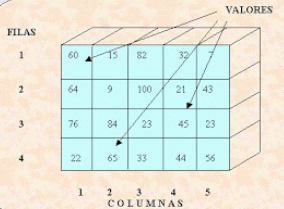
\includegraphics[scale=0.5]{2bidimensional}
\end{figure}

int cubo[2,2,8]
\begin{figure}[H]
  \centering
  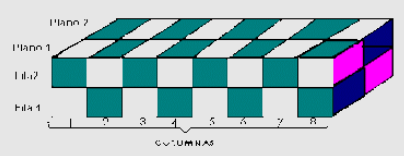
\includegraphics[scale=0.5]{2tridimensional}
\end{figure}

Estas estructuras las podemos trabajar con instrucciones como:

\begin{verbatim}
matriz[3,2] = 0 ;
o
int x = cubo [1,2,4] * 3 ;
\end{verbatim}

Sin embargo, debemos tomar en cuenta que, aunque el lenguaje nos
permita realizar este acceso fácilmente, la memoria de la computadora
no es multidimensional, y las matrices, cubos y arreglos de más de 3
dimensiones, deben poder mapear cada uno de los elemento, con una
coordenada única (conjunto de índices).

Esto implica que cada elemento debe tener un orden definido, de forma
que sea posible accederlo de forma inequívoca.  Dicho orden es el
orden lexicográfico:

\begin{definicion}
  \textbf{Orden lexicográfico por fila}: la posición ($a_1$, $a_2$
  ,..., $a_k$) es menor que ($b_1$, $b_2$,..., $b_k$), si y sólo si
  para algún $1 < j \leq k$, existe un $i$ tal que $a_i$ = $b_i$, para
  $1 \leq i < j$, y $a_j$ < $b_j$
\end{definicion}

Por ejemplo: si tenemos las coordenadas A=(1, 5, 1, 9) y B = (1, 5, 2,
8), el orden lexicográfico nos dice que A< B. En este caso k = 4,
entonces necesitamos un número entre 1 y 4 (la variable j), que sea el
índice de la coordenada tal que las coordenadas anteriores sean
iguales en A y B, y $a_j$ sea menor a $b_j$. En este caso, ese número
j corresponde a 3. Nótese que en la primera y segunda coordenada
tienen el mismo valor, y en la tercera se cumple que 1<2.

Dado que tenemos las dimensiones de una arreglo, y su dirección
inicial, es factible calcular la posición de cualquier elemento, dada
sus coordenada.  Lo cual veremos del caso más simple al caso general.

\subsection{Caso unidimensional}
\label{sec:caso-unidimensional}

Supongamos el siguiente vector $V$ de 4 elementos\\

\hspace{1in} $V: 1 .. 4$

\begin{center}
  \begin{tabular}{|c|c|c|c|}
    \hline
    1 & 2 & 3 & 4\\ \hline
  \end{tabular}
\end{center}

¿cuál sería la fórmula que nos permita mapear cualquier elemento de
este vector?  $Loc \left(V[i] \right)$ = ?

Por ejemplo: encontrar el elemento $V[3]$. Aquí, la dirección del
primero elemento es

$$ \alpha = \&V[1]$$

y

$$Loc \left( V[3] \right) =  \alpha + 2$$

Para encontrar el elemento $V[i]$

$$Loc \left( V[i] \right) = \alpha + i - 1$$

Si cambiamos la definición de $V$ a\\

\hspace{1in} $V:\; 10..13$

\begin{center}
  \begin{tabular}{|c|c|c|c|}
    \hline
    10 & 11 & 12 & 13\\ \hline
  \end{tabular}
\end{center}

aquí, la dirección del primero elemento es

$$ \alpha = \&V[10]$$

Entonces, para encontrar el elemento $V[12]$, ya no nos funcionaría la
fórmula anterior, dado que el índice inicial cambia de 1 a 10, por lo
tanto tenemos que cambiar a:

$$Loc \left( V[12] \right) = \alpha + 12 - 10$$

En general si tenemos un vector $V$ con pares límites arbitrarios así:

$$V: n_1..m_1$$

aquí, la dirección del primero elemento es

$$ \alpha = \&V[n_1]$$

Entonces, la fórmula cambia así:

$$ Loc \left( V[i] \right) =  \alpha + i - n_1$$

\subsection{Caso bidimensional}
\label{sec:caso-bidimensional}

Para el caso de una matriz (arreglo bidimensional), de 3*4 definida
como:

$$M:\; 1..3 * 1..4$$

aquí, la dirección del primero elemento es

$ \alpha = \&M[1,1]$

La conceptualizamos así:

\begin{center}
  \begin{tabular}{|c|c|c|c|}
    \hline
    1,1 & 1,2 & 1,3 & 1,4\\ \hline
    2,1 & 2,2 &	\textbf{2,3} & 2,4\\ \hline
    3,1 & 3,2 &	3,3 & 3,4\\ \hline
  \end{tabular}
\end{center}

Pero en memoria, realmente queda así:
\begin{center}
  \begin{tabular}{|c|c|c|c|c|c|c|c|c|c|c|c|}
    \hline
    1,1&1,2&1,3&1,4&2,1&2,2&\textbf{2,3}&2,4&3,1&3,2&3,3&3,4\\ \hline
  \end{tabular}
\end{center}

¿cuál sería la fórmula que nos permita mapear cualquier elemento de
esta matriz?  Si queremos encontrar el elemento M[2,3].

$$Loc \left( M[2,3]  \right) = \alpha + ?$$

Dado que el elemento está en la fila 2, sabemos que se debe avanzar
totalmente la primera fila (avanzarAFila), y luego aplicamos al
fórmula del vector, ya que cada fila es un vector.  Así:

$$Loc \left( M[2,3] \right) = \alpha + avanzarAFila(2) + 3 - 1$$

De esta forma tenemos que avanzar 4 elementos, ya que cada fila es de
tamaño 4.

$$ Loc \left( M[2,3] \right) = \alpha + 1 * 4 + 3 - 1 $$

Generalizando un poco más, si en esta matriz queremos encontrar un
elemento arbitriario $A[i,j]$ , aplicamos la fórmula así:

$$ Loc \left( M[2,3] \right) = \alpha + avanzarAFila(i) +  (j - 1) $$

Es decir debemos avanzar las filas necesarias para llegar a la fila $i$
y luego dentro de esa fila aplicamos la fórmula para un vector.

En general \textbf{\em avanzarAFila(i)}, se compone de dos elemento:
$FilasAntesDe(i) * TamanoDeCadaFila$, que en este caso son

\begin{eqnarray*}
  Loc \left( M[2,3] \right) &=& \alpha + FilasAntesDe(i)*TamanoDeCadaFila +  (j - 1)\\
  &=& \alpha + (i-1)*(4) +  (j - 1) 
\end{eqnarray*}

En general, si $M$ tiene pares límites arbitrarios, definida así:
$$M:\; n_1..m_1*n_2..m_2$$

aquí, la dirección del primero elemento es
$$\alpha = \&M[n_1,n_2]$$

y la fórmula cambia a:
\begin{eqnarray*}
Loc \left( A[i_1,i_2] \right) &=& \alpha + avanzarAFila(i_1) +  (i_2 - n_2)\\
&=&\alpha + FilasAntesDe(i_1)*TamanoDeCadaFila +  (i_2 - n_2)
\end{eqnarray*}

Dado que el límite inferior de la primera dimensión es $n_1$ entonces
$$FilasAntesDe(i_1) = i_1 - n_1$$

y, el tamaño de cada fila está dado por los límites de las columnas,
entonces
$$TamanoDeCadaFila = m_2 - n_2  + 1$$

Por lo tanto, la fórmula queda
$$Loc \left( A[i_1,i_2] \right) = \alpha + (i_1 - n_1)*(m_2 - n_2  + 1)  +  (i_2 - n_2)$$

\subsection{Caso tridimensional}
\label{sec:caso-tridimensional}
Sea el cubo

$$ C:\; 1..3 * 1..4 * 1..2 $$

aquí, la dirección del primer elemento es

$$ \alpha = \&C[1,1,1]$$

Tener en cuenta que en este caso, tenemos que cada índice en la
primera dimensión representa una matriz y cada índice en la segunda
dimensión, representa una fila de la matriz correspondiente, y la
última dimensión representa un elemento individual.

Así, se se desea acceder el elemento A[2,3,2], aplicamos la siguiente
deducción

\begin{eqnarray*}
  Loc \left( C[2,3,2] \right) &=& \alpha + avanzarAMatriz(2) + AvanzarAFila(3) +  (2 - 1)\\
  &=& \alpha + MatricesAntesDe(2)*TamanoDeCadaMatriz \\
  & & + FilasAntesDe(3)*TamanoDeCadaFila + (1)
\end{eqnarray*}

Sabemos que

$$ TamanoDeCadaMatriz = Filas * Columnas = 4 * 2 = 8 $$

y

$$ MatricesAntesDe(2) = 1 $$

y

$$TamanoDeCadaFila=2$$

y

$$ FilasAntesDe(3) = 2 $$

Por lo tanto

$$Loc \left( C[2,3,2] \right) = \alpha + (1)*8 + (2)*2 + (1) = \alpha + 13$$

En general, si C tiene pares límites arbitrarios,  así:

$$C: n_1..m_1 * n_2..m_2 * n_3..m_3$$

aquí, la dirección del primero elemento es

$$ \alpha = \&C[n_1, n_2, n_3]$$

y la fórmula cambia a:
\begin{eqnarray*}
  Loc \left( C[i_1, i_2, i_3] \right) &=& \alpha + avanzarAMatriz(i_1) + AvanzarAFila(i_2) \\
  & & + AvanzarAlElemento(i_3)\\
  \\
  &=& \alpha+\textcolor{red}{MatricesAntesDe(i_1)}*\textcolor{blue}{TamanoDeCadaMatriz}\\
  & &+\textcolor{cyan}{FilasAntesDe(i_2)} * \textcolor{green}{TamanoDeCadaFila}+(i_3-n_3)\\
  \\
  &=& \alpha + \textcolor{red}{(i_1-n_1)}* \textcolor{blue}{(m_2-n_2+1)*(m_3-n_3+1)}\\
  & &+\textcolor{cyan}{(i_2-n_2)}*\textcolor{green}{(m_3-n_3+1)}+(i_3-n_3)
\end{eqnarray*}

\subsection{Caso k-dimensional}
\label{sec:caso-k-dimensional}

Sea el siguiente arreglo k-dimensional

$$A:\;n_1..m_1 * n_2..m_2 * ... * n_k..m_k$$

aquí, la dirección del primero elemento es

$$ \alpha = \&A[n_1, n2,..., n_k]$$

Entonces deducimos la fórmula así:

\begin{eqnarray*}
  Loc \left( A[i_1, i_2, ... ,i_k] \right) &=& \alpha + ElementosDimension_1AntesDe(i_1)\\
  & & + ElementosDimension_2AntesDe( i_2)+ .... \\
  & & + ElementosDimension_{k-1}AntesDe (i_{k-1}) \\
  & & + AvanzarAlElemento(i_k)
\end{eqnarray*}

Sabemos que
$$ElementosDimension_xAntesDe(i_x) = (i_x -  n_x) * TamanoDeCadaElementoEnDimension_x$$

y para calcular el $TamanoDeCadaElementoEnDimension_x$ , revisemos los
casos anteriores:

\begin{description}
\item[Tamaño de cada elemento en la última dimensión: ]
  $$1$$
\item[Tamaño de la ultima fila (dimensión k-1): ]
  $$ m_k - n_k + 1$$
\item[Tamaño de la última matriz ( dimension k -2 ): ]
  $$(m_{k-1} - n_{k-1} + 1) * (m_k - n_k + 1) $$
\item[Tamaño del último cubo (dimensión k-3): ]
  $$(m_{k-2} - n_{k-2} + 1) * (m_{k-1} - n_{k-1} + 1) * (m_k - n_k + 1) $$
\item[...]
\item[Tamaño de la dimensión k-j: ]
  $$(m_{k-j+1} - n_{k-j+1} +1) * ...* (m_{k-1} - n_{k-1} + 1) * (m_k - n_k + 1) $$
\item[...]
\item[Tamaño de la primera dimensión (cuando k-j=1 y k-j+1=2): ]
  $$(m_2 - n_2 +1) * ...* (m_{k-1} - n_{k-1} + 1) * (m_k - n_k + 1)$$
\end{description}

Por lo tanto:
\begin{eqnarray*}
  Loc (A[i_1, i_2, ... ,i_k]) &=& \alpha + (i_1 - n_1) *(m_2 - n_2 -1) * ...* (m_{k-1} - n_{k-1} + 1) * (m_k - n_k + 1)\\
  & & + (i_2 - n_2) *(m_3 - n_3 -1) * ...* (m_{k-1} - n_{k-1} + 1) * (m_k - n_k + 1)\\
  & & + (i_3 - n_3) *(m_4 - n_4 -1) * ...* (m_{k-1} - n_{k-1} + 1) * (m_k - n_k + 1)\\
  & & +.........+\\
  & & + (i_{k-1} - n_{k-1}) * (m_k - n_k + 1)\\
  & & + (i_k - n_k) 
\end{eqnarray*}

\[
Loc (A[i_1, i_2, ... ,i_k])= \alpha + \sum_{x=1}^k \left[(i_x-n_x) \prod_{y=x+1}^k\left(m_y-n_y+1\right)\right]
\]

\subsubsection{Ejemplo}
\label{sec:ejemplo}

\begin{definicion}
  \textbf{Orden lexicográfico por columna}. La posición $(a_1, a_2 ,
  \ldots , a_k)$ es menor que $(b_1, b_2, \ldots , b_k)$, si y sólo si
  para algún $1 < j \leq k$, existe un $i$ tal que $a_i = b_i$, para
  todo $j < i \leq k$, y $a_j < b_j$
\end{definicion}

$$\text{Ej.} Matriz:\; 1..3 * 1..4$$
\begin{center}
  \begin{tabular}{|c|c|c|c|}
    \hline
    1,1 & 1,2 & 1,3 & 1,4\\ \hline
    2,1 & 2,2 &	\textbf{2,3} & 2,4\\ \hline
    3,1 & 3,2 &	3,3 & 3,4\\ \hline
  \end{tabular}
\end{center}

Se almacena así:
\begin{center}
  \begin{tabular}{|c|c|c|c|c|c|c|c|c|c|c|c|}
    \hline
    1,1&1,2&1,3&1,4&2,1&2,2&\textbf{2,3}&2,4&3,1&3,2&3,3&3,4\\ \hline
  \end{tabular}
\end{center}

sea $A$ un arreglo de $n_1..m_1 * n_2..m_2$ ordenado
lexicográficamente por columnas. Deducir $LOC \left( A[i,j] \right) =
\alpha + (j-n_2) * (m_1-n_1+1) + (i-n_1)$

En general, para el arreglo $A:\; n_1..m_1 * n_2..m_2 * .... * n_k..m_k$

\begin{eqnarray*}
  LOC \left( A[i_1, i_2, .., ik] \right) &=& \alpha + (i_k - n_k)* (m_1 - n_1 +1) * (m_2 - n_2 + 1) * ...* (m_{k-1} - n_{k-1}  +1 )\\
  & & + (i_{k-1} - n_{k-1} ) * (m_1 - n_1 +1) * (m_2 - n_2 + 1) * ...* (m_{k-2} - n_{k-2}  +1 ) + \\
  & &  \ldots \\
  & &  (i_2 - n_2 ) * (m_1 - n_1 +1)  + \\
  & & (i_1 - n_1 )
\end{eqnarray*}




\section{Arreglos esparcidos}
Vimos que el uso de arreglos lexicográficos tiene el mejor rendimiento
posible (constante) para el acceso de elementos por índice.  Sin
embargo, el hecho de que necesiten reservar memoria contigua para
todos sus posibles elementos, implica que existen situaciones en las
que no son recomendables, debido principalmente a dos factores:

\begin{enumerate}
\item Desperdicio de memoria: consideremos una matriz de 1,000 por 1,000
elementos, de los cuales sólo se están utilizado 10. Sería un gran
desperdicio de memoria, alojar 1,000,000 de elementos para sólo
utilizar 10.
\item Incapacidad de alojar espacio para todos los posibles elementos: las
hojas electrónicas tienen una gran capacidad de celdas, pero
normalmente sólo se utiliza una pequeña porción de ellas: Excel tiene
su máxima celda en IV65536, lo que significa una capacidad para
(26*8+22)*65536 = 15,073,280 celdas.  Si cada una de estas ocupara 1
byte, no tendríamos memoria suficiente para una hoja electrónica..
\end{enumerate}


En cualquiera de estos casos resultan útiles los arreglos esparcidos,
los cuales tienen como característica fundamental que \textbf{sólo utilizan la
memoria realmente necesaria conforme se agregan elementos al arreglo}.

\subsection{Técnicas de representación}

Entre muchas técnicas para lograr los arreglos esparcidos,
distinguiremos dos principales:
\begin{itemize}
\item Arreglos lexicográficos de encabezados, con celdas de referencias cruzadas.
\item Listas de encablezados
\end{itemize}

El uso de arreglos lexicográficos para los encabezados se ilustran en
la siguiente figura:
\begin{figure}[H]
  \centering
  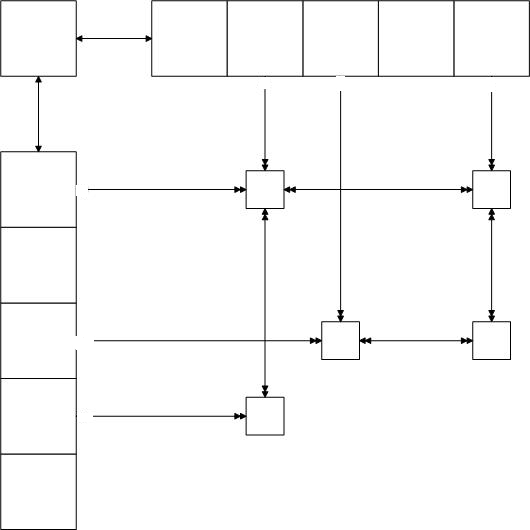
\includegraphics[scale=0.6]{3arregloLexografico}
\end{figure}

Se tiene un control de encabezados, el cual contiene dos apuntadores:
uno para el arreglo de las filas y el otro para las columnas.  Los
encabezados no necesitan más información que el apuntador al primer
nodo de la fila o columna.  Cada uno de los nodos tiene la siguiente
estructura:
\begin{figure}[H]
  \centering
  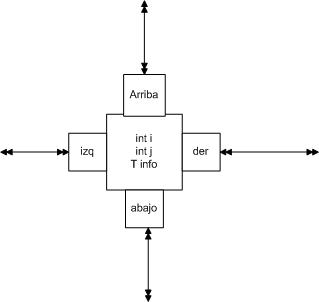
\includegraphics[scale=0.7]{3nodo.jpeg}
\end{figure}

Los cuatro apuntadores de navegación nos sirven para facilitar los
recorridos y búsqueda de cada nodo.  Notemos que, además de la info,
se debe tener en cada nodo la información de los índices que
representan, ya que la caraterística de esparcido no permite calcular
el índice de un nodo basado en sus posición de forma fácil.  Se podría
omitir esta información, para para buscar cada nodo implicaría una
doble búsqueda, por fila y columna, para cada nodo, lo cual lo haría
muy ineficiente.

La estrategia básica del algoritmo de localización de un elemento
A[i,j]

\begin{alltt}
   {\it Seleccionar el encabezado de las filas, aunque también puede ser por columna
   Para cada nodo en la lista de la fila {\bf i}}
  
   Si {\bf nodo.j < j}
        nodo = nodo.der  ; {\it //seguimos buscando}
   sino
        si {\bf nodo.j=j}
             return {\bf nodo} ; {\it // encontramos el nodo}
        {\bf sino}
             return null ;  {\it // no se encuentra el nodo con los índices indicados}
        fin
   fin 
\end{alltt}

Una implementación más formal, podría ser la siguiente:

\begin{verbatim}
public class ArregloEsparcido<E> extends ArregloGeneral<E> {
.
.
.
       public  E get (int i[]) {
            /* resumiendo a búsqueda por filas */
            Nodo n = fila [i] ;

            while (n != null &&  n.col < j) {
                n = n.derecha ;
            }
            if ( n == null )
                return null ;
            else
                return n.obj ;
       }
.
.
.
}
\end{verbatim}

Analizando el orden de este algoritmo:
\begin{itemize}
\item El peor de los casos es una matriz de una solo fila, la cual está
llena y estamos buscando el último elemento de dicha fila.  En este
caso el O(get(i)) = n, es decir lineal, ya que visitaremos todos los
elementos.
\item Si fuera una matriz cuadrada totalmente llena, entonces n = filas *
columnas y filas = columnas = x , por lo tanto $n = x^2$ .  Al hacer la
búsqueda del último elemento de cada fila, recorreremos x elementos,
es decir O(get(i)) = sqrt(n).
\item En el caso general, en que las filas != columnas, O(get(i)) =
  n/columnas, es decir se convierte en sublineal.
\end{itemize}

Por lo tanto el orden de este algoritmo varia de lineal a sublineal,
dependiendo de la estructura de la matriz.

Las otra técnica de representación está basada en que también los
encabezados son listas, en vez de arreglos lexicográficos.  Así, otra
representación de la matriz anterior es así:
\begin{figure}[H]
  \centering
  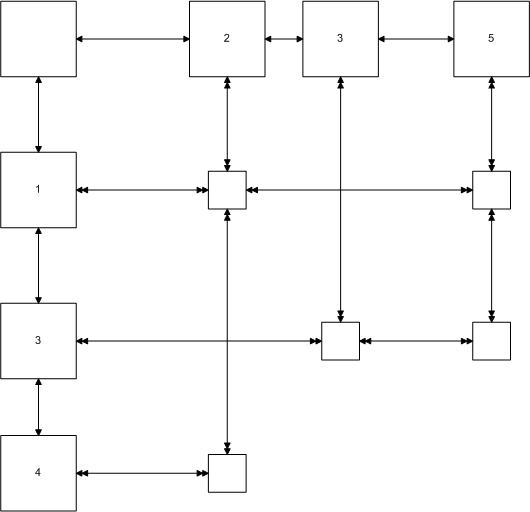
\includegraphics[scale=0.5]{3encabezadosLista.jpeg}
\end{figure}

Aquí los nodos de los encabezados tendrían la siguiente estructura:
\begin{figure}[H]
  \centering
  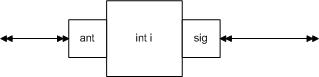
\includegraphics[scale=0.8]{3nodoEncabezadoLista.jpeg}
\end{figure}

Esta representación al seguir manteniendo los nodos con doble enlace
en ambas dimensiones, permite tener la misma flexibilidad en el
recorrido de elementos que la representación con encabezados de
arreglos.  La diferencia básica es que el recorrido en los
encabezados.  Sin embargo, cuando se tienen múltiples dimensiones,
mantener en los nodos el doble enlace hacia cualquier dirección,
complica de gran manera las operaciones de inserción y eliminación,
además de representar un consumo alto de memoria por uso de dos
apuntadores por nodo, por dimensión.  Para estos casos se podría
utilizar una representación como la siguiente:

\begin{center}
  arreglos-ortogonales-listas2
\end{center}

En este caso, los nodos de información ya no necesitan almacenar ni
apuntadores, ni índices de la posición que representa, ya que dicha
posición, es determinada en el recorrido de los encabezados.

El almacenamiento encadenado puede ser útil para acomodar el
crecimientos de los arreglos en direcciones arbitrarias, a costa de de
una utilización de espacio reducido

\subsection{Comparación de técnicas}
\label{sec:comp-de-tecn}

El rendimiento del acceso a los arreglos, está dado por la
representación interna

\subsubsection{Criterios de comparación}
\label{sec:crit-de-comp}

\begin{itemize}
\item simplicidad de acceso a los elementos
\item facilidad de recorridos en diferentes rutas
\item eficiencia de uso del almacenamiento
\item facilidad de crecimiento
\end{itemize}

\subsubsection{Almacenamiento lexicográfico vs esparcido}
\label{sec:almac-lexic-vs}

\paragraph{Ventajas}
\label{sec:ventajas}

\begin{itemize}
\item cálculo fácil ( O(n) = c )
\item facilidad de recorrido
\item crecimiento fácil en la primera dimensión
\end{itemize}

\paragraph{Desventajas}
\label{sec:desventajas}

\begin{itemize}
\item crecimiento muy costos en las otras dimensiones
\item Uso de la memoria sólo es óptimo si está lleno (o casi lleno).
  Radio = ( tam(objeto) / tam(objeto + apuntadores) ) indica el máximo
  porcentaje de llenado a partir del cual es más eficiente un arreglo
  lexicográfico.
\end{itemize}



%%% Local Variables:
%%% TeX-master: "tedd"
%%% End:


% expresiones regulares, en su momento,  utiles para este doc:
% \([[:alpha:]]\)\([[:digit:]]\) -> \1_\2


\chapter{Árboles}
\label{cha:arboles}
Conceptos generales y representaciones de árboles
\section{ Conceptos generales de árboles }
\subsection{La teoría de grafos y los árboles}
El concepto de \textbf{árbol} como estructura de datos tiene su origen en el
concepto de grafo.  Repasando, a continuación algunos conceptos de
grafos:

\begin{itemize}
\item \textbf{Grafo}: es una colección de de vértices $V$, y una
  colección de lados $L$, donde por cada lado en $L$, hay una línea
  que une un par de vértices en $V$
\item \textbf{Vértices Adyacentes}: son los que están unidos por un
  lado
\item \textbf{Ruta}: de longitud $n$, es una secuencia de lados $l_1
  l_2 \dotso l_n$, donde lado $l_k$ comparte un vértice en común con
  el lado precedente $l_{k-1}$, y un vértice en común con el lado
  subsiguiente $l_{k+1}$, para $1 < k < n$. Otra definición es: Ruta
  de longitud $n$ es un conjunto de vértices $v_0v_1 \ldots v_n$, tal
  que $v_{k-1}$ es adyacente a $v_k$, para $1 < k < n$.
\item \textbf{Ruta Simple}: cuando todos los vértices en él son
  distintos, excepto posiblemente por el primero y último
\item \textbf{Ciclo}: es una ruta de longitud tres o más, que conecta
  un vértice $v$ con él mismo.
\item \textbf{Ciclo Simple}: es un ciclo, cuya ruta es simple.
\item \textbf{Grafo Conectado}: es aquel donde existe, al menos una
  ruta de un vértice a otro.
\item \textbf{Árbol libre}: es un grafo finito y conectado, sin ciclos
  simples.
\item \textbf{Árbol orientado}: es un grafo, donde cada lado de $L$,
  es un par de vértices de la forma $(v, v’)$ donde se dice que $v$ es
  el origen y $v’$ es el destino y la dirección de $l$ va de $v$ a
  $v’$, y se toma un vértice $r$ como la raíz donde inicia el grafo.
\item \textbf{Árbol ordenado}: es un conjunto finito de uno o más
  vértices tales que hay un vértice designado $r$, llamado la raíz, y
  tal que los vértices restantes, son divididos en $n > 0$
  subconjuntos mutuamente exclusivos, cada uno de los cuales son a la
  vez árboles ordenados.
\item \textbf{Árbol binario}: Es un conjunto finito de vértices que
  están vacíos o consiste de un vértice llamado raíz y dos subárboles
  binarios, los cuales son disjuntos uno del otro, y son llamados
  subárboles izquierdo y derecho
\item \textbf{Árbol binario lleno}: Es un árbol binario en el cual
  cada nodo o es hoja o tiene exactamente dos descendientes no vacíos.
\item \textbf{Árbol binario completo}: es un árbol binario con hojas
  en los dos últimos niveles y en las hojas del último nivel están a
  la izquierda
\end{itemize}

Los árboles como estructuras de datos son sólo una de las aplicaciones
que existen para este concepto.  Entre ellos están los \textbf{árboles de
costo mínimo}, los \textbf{árboles de expresiones}, \textbf{mapas}, etc.

\subsection{Representaciones de árboles en memoria}
\label{sec:repr-de-arbol}

Los árboles binarios son construidos típicamente con una estructura de
nodos y apuntadores en la cual se almacenan datos, cada uno de estos
nodos tienen una referencia o apuntador a un nodo izquierdo y a un
nodo derecho denominados hijos. En ocasiones, también contiene un
apuntador a un único nodo. Si un nodo tiene menos de dos hijos,
algunos de los punteros de los hijos pueden ser definidos como nulos
para indicar que no dispone de dicho nodo. En la figura adjunta se
puede observar la estructura de dicha implementación.

\begin{figure}[H]
  \centering
  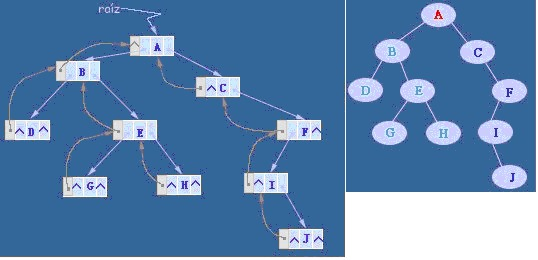
\includegraphics[scale=.5]{1arbolEnMemoria.jpg}
  \caption{Árbol en memoria}
  \label{fig:1arbolEnMemoria}
\end{figure}

Los árboles binarios también pueden ser almacenados como una
estructura de datos implícita en arrays, y si el árbol es un árbol
binario completo, este método no desaprovecha el espacio en
memoria. Tomaremos como notación la siguiente: si un nodo tiene un
índice $i$, sus hijos se encuentran en índices $2i+1$ y $2i + 2$,
mientras que sus padres (si los tiene) se encuentra en el índice
$(i-1)/2$ (partiendo de que la raiz tenga índice cero). Este método
tiene como ventajas el tener almacenados los datos de forma más
compacta y por tener una forma mas rápida y eficiente de localizar los
datos en particular durante un preoden transversal. Sin embargo, \textit{si el
árbol no está completo, desperdicia mucho espacio en memoria}.
\begin{figure}[H]
  \centering
  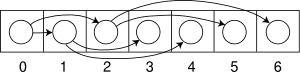
\includegraphics[scale=.7]{2arbolBinarioEnArray.jpg}
  \caption{Árbol binario en array.}
  \label{fig:2arbolBinarioEnArray}
\end{figure}

\subsection{Codificación de árboles n-arios como árboles binarios}
\label{sec:codif-de-arbol}
Hay un mapeo uno a uno entre los arboles generales y arboles binarios,
el cual en particular es usado en Lisp para representar arboles
generales como arboles binarios. Cada nodo $N$ ordenado en el árbol
corresponde a un nodo $N'$ en el árbol binario; el hijo de la
izquierda de $N'$ es el nodo correspondiente al primer hijo de $N$, y
el hijo derecho de $N'$ es el nodo correspondiente al siguiente
hermano de $N$, es decir, el próximo nodo en orden entre los hijos de
los padres de $N$.

Este representación de árbol binario de un árbol general, a veces se
hace referencia como un árbol binario \textbf{primer hijo/siguiente hermano}, o
un árbol doblemente encadenado.

Una manera de pensar acerca de esto es que los hijos de cada nodos
esten en una lista enlazada, encadenados junto con campo derecho, y el
nodo sólo tiene un \textbf{apuntador} al comienzo o la cabeza de esta
lista, a través de su campo izquierdo.

Por ejemplo, en el árbol de la izquierda, la A tiene 6 hijos (B, C, D,
E, F, G). Puede ser convertido en el árbol binario de la derecha.
\begin{figure}[H]
  \centering
  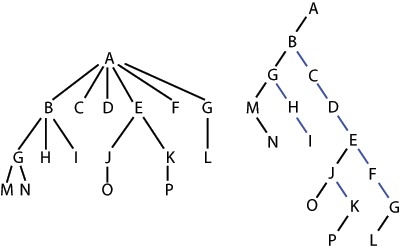
\includegraphics[scale=2]{3arbolGeneralABinario.jpg}
  \caption{Árbol general a binario}
  \label{fig:3arbolGeneralABinario}
\end{figure}

Esta representación tiene la ventaja que puede representar cualquier
árbol multihijos, utilizando sólo dos apuntadores por nodo.  Es útil
cuando el árbol a representar tiene una gran cantidad de hijos por
nodo, o la cantidad de hijos es variable y/o indeterminada.

La desventaja es que los recorridos se complica.

\section{Operaciones sobre árboles}
\label{sec:oper-sobre-arbol}

Como estructura de datos, sobre los árboles se pueden realizar
diferentes operaciones como agregar, buscar y eliminar elementos del
árbol.  Sin embargo cualquier problema que se quiera resolver con el
uso de árboles, en general, se convertirá en realizar un
\textbf{recorrido} sobre el árbol.

\subsection{Recorridos}
\label{sec:recorridos}
\begin{definicion}
  Un \textbf{recorrido} es una operación sobre un árbol en el que se
  recorren los elementos en algún orden definido, para realizar sobre
  los elementos algún proceso, llamado VISITA.
\end{definicion}

Según esta definición, hay $n!$ formas de recorrer un árbol con n
elementos, lo cual nos deja un número igual de recorridos posibles.
Sin embargo, las operaciones de recorrido definidas se refieren
normalmente a \textbf{recorridos completos}.

\begin{definicion}
  Un \textbf{recorrido completo} es un tipo de recorrido en el cual se
  VISITAN todos elementos del árbol, en algún orden definido.
\end{definicion}


Existen varios recorridos definidos, pero veremos cuatro principales.
Así, sea un árbol T con subarbol izquierdo Ti y subarbol derecho Td,
entonces se tienen los siguientes recorridos

\begin{description}
\item[Preorden: ] es el recorrido donde se VISITA T y luego se realiza
  el recorrido preorden de Ti y luego el recorrido preorden de Td
\item[En orden: ] es el recorrido donde se realiza el recorrido en
  orden de Ti, y luego se VISITA T y luego el recorrido en orden de Td
\item[Postorden: ] es el recorrido se realiza el recorrido post orden
  de Ti, luego el recorrido post orden de Td y luego se VISITA T
\item[Por niveles: ] es el recorrido donde se VISITAN los nodos en el
  orden del nivel del árbol, así se visita T, luego se realiza el
  recorrido de las raices de Ti y Td, luego el recorrido por nivel de
  los hijos inmediatos de Ti y Td, y así sucesivamente hasta recorrer
  todos los niveles.
\end{description}

Cada uno de estos recorridos produce una secuencia de elementos que
toma el nombre del recorrido correspondientes.  Así hablamos de la
\textit{secuencia preorden}, \textit{secuencia en orden}, etc.
Por ejemplo: en el siguiente árbol
\begin{figure}[H]
  \centering
  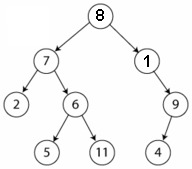
\includegraphics[scale=.6]{4arbolSecuencias.jpg}
  \caption{Secuencias de un árbol.}
  \label{fig:4arbolSecuencias}
\end{figure}

Tiene las siguientes secuencias:


\begin{itemize}
\item Secuencia pre orden: 8, 7, 2, 6, 5 , 11, 1, 9, 4
\item Secuencia en orden: 2, 7, 5, 6, 11, 8, 1, 4, 9
\item Secuencia post orden: 2, 5, 11, 6, 7, 4, 9, 1, 8
\item Secuencia por niveles: 8, 7, 1, 2, 6, 9, 5, 11, 4
\end{itemize}

En cada secuencia de llaves, que determina una relación de sucesor y
predecesor en cada recorrido, así hablamos de relaciones
sucesor-predecesor, según las secuencias.  Por ejemplo: 5 es
predecesor en preorden del 11, predecesor en orden del 6, sucesor en
postorden del 2

Una posible implementación es:

\begin{verbatim}
class NodoBin {
   NodoBin *izq ;
   NodoBin *der ;
   TInfo info ;
   .....
}

class ArbolBinario {
   public:
      void preOrden () {
         preOrden(raiz) ;
      }

      void enOrden () {
         enOrden(raiz) ;
      }


      void postOrden () {
         postOrden(raiz) ;
      }
   private:
      NodoBin *raiz ;
      ....
      void visita (NodoBin *n) {
          // cualquier operación que se desee hacer sobre cada nodo
      }

      void preOrden (NodoBin *n) {
         if  ( n != null) {
            visita (n) ;
            preOrden(n->izq) ;
            preOrden(n->der) ;
         }
      }

      void enOrden (NodoBin *n) {
         if  ( n != null) {
         enOrden(n->izq) ;
         visita (n) ;
         enOrden(n->der) ;
         }
      }

      void postOrden (NodoBin n) {
         if  ( n != null) {
            postOrden(n->izq) ;
            postOrden(n->der) ;
            visita (n) ;
         }
      }
} 
\end{verbatim}

\section{Árboles binarios de búsqueda}
\label{sec:arboles-binarios-de}

Un árbol de búsqueda, también de comparación o decisión, es un árbol
en el que cada llave $L$ tiene subárbol izquierdo y derecho, tal que las
llaves del subárbol izquierdo de $L$ son menores a $L$, y las del subárbol
derecho son mayores a $L$, y los subarboles derecho e izquierdo de $L$ son
también árboles de búsqueda.

Nótese que hablamos de llaves en vez de nodos

\subsection{Árbol binario de búsqueda}
\label{sec:arbol-binario-de}
Es un árbol de búsqueda en el que cada nodo tiene si mucho 2 hijos.

Por ejemplo, en la siguiente gráfica tenemos el árbol binario
anterior, convertido en árbol binario de búsqueda:

\begin{figure}[H]
  \centering
  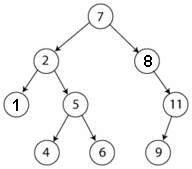
\includegraphics[scale=0.5]{5arbolBusquedaBinaria.jpg}
  \caption{Árbol binario de busqueda de Figura \ref{fig:4arbolSecuencias}}
  \label{fig:5arbolBusquedaBinaria}
\end{figure}

 Otro ejemplo:
\begin{figure}[H]
  \centering
  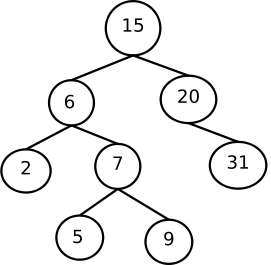
\includegraphics[scale=0.4]{6otroArbolBusquedaBinaria.jpg}
  \caption{Otro árbol binario de busqueda.}
  \label{fig:6otroArbolBusquedaBinaria}
\end{figure}

\subsection{Búsqueda}
\label{sec:busqueda}

La búsqueda consiste acceder a la raíz del árbol, si el elemento a
localizar coincide con éste la búsqueda ha concluido con éxito, si el
elemento es menor se busca en el subárbol izquierdo y si es mayor en
el derecho. Si se alcanza un nodo hoja y el elemento no ha sido
encontrado se supone que no existe en el árbol. Cabe destacar que la
búsqueda en este tipo de árboles es muy eficiente, representa una
función logarítmica de base 2.
\begin{verbatim}
class NodoBin {
   TLlave llv ;
   TValor value
   NodoBin *izq, *der ;

   NodoBin (TLlave llv, TValor value) {
      this->llv = llv ;
      this->value = value ;
      izq = null ;
      der = null ;
   }
}

class ArbolBinBusqueda :: ArbolBinario {
   NodoBin *raiz ;
   .....
   TValor get(TLlave llv) {
      NodoBin * temp = raiz ;

      while ( temp != nullptr && llv != temp.llv) {
         if (llv < temp->llv) {
            temp = temp->izq ;
         }else{
            temp = temp->der ;
         }
      }

      if ( temp == null)
          return null ; // no está
      else
          return temp.valor ;
   }
} 
\end{verbatim}

\textbf{Uso correcto de clases}: En general, cuando trabajamos
programación orientada a objetos, se comete el error común de
saltarnos un método de una clase.  Usualmente tenemos un método como
el siguiente:
\begin{verbatim}
class x {
   ....
   int x1(T obj) {
      if ( obj.a() )
          x = obj.b() ;
      ....
      obj.c() ;
      ..
      obj.d() ;
      ..
   }
   ...
   int y() {
      ...
      x1(o) ;
      ..
   }
} 
\end{verbatim}

Nos damos cuenta que en el método \textbf{x1}, se se recibe un
parámetro del clase \textbf{T}, y toda la lógica del método es
alrededor de dicho parámetro (\textbf{obj}), entonces ésto debería
convertirse en:
\begin{verbatim}
class T {
   int x1() {
      if (a() ) ..
         x = b() ;
      c() ;
      ..
      d() ;
      ..
   }
   ....
}

class x {
   ...
   int y() {
      ...
      o.x1() ;
      ..
   }
}
\end{verbatim}

\subsection{Orden de la búsqueda}
\label{sec:orden-de-la}

\begin{eqnarray*}
  \label{eq:1}
  T(get(n)) &=& T(asignacion) + T(while) + T(if) ;\\
    &=& t + ( T(condicion) + K * T(cuerpo) ) + ( T(condicion) + max ( T(then) , T(else) )  )\\
    &=& t + ( t + K ( T(if) ) ) + ( t + max ( t, t ) ) \\
    &=& t + ( t + K ( T(condicion) + max ( T(then) , T(else) )) ) + ( t +  t ) \\
    &=& t + ( t + K ( t + max ( t , t )) ) + ( t +  t ) \\
    &=& t + ( t + K ( t + t ) + ( t +  t ) 
\end{eqnarray*}

$K$ es el número de veces que se ejecuta el cuerpo del while, en
términos de $n$, donde $n$ es el número de llaves.

$K$ = altura del arbol y la relación entre la altura y $N$ está dada por  
\[ 2^k - 1 = n  \longrightarrow   k = lg ( n + 1)\]

por lo tanto
\begin{eqnarray*}
  \label{eq:2}
  T(get(n)) &=&  t + ( t + lg ( n + 1) ( t + t ) + ( t +  t ) \\
    &=& 4t + lg ( n + 1) ( 2t + t ) \longrightarrow O(get(n)) = lg(n) 
\end{eqnarray*}

\subsection{Inserción}
\label{sec:insercion}

La inserción es similar a la búsqueda. Se procede de la siguiente
forma, si el nodo pasado como parámetro está vacío se crea un nuevo
nodo para él cuyo contenido correspondiente sería el elemento a
insertar. Si no lo está, se comprueba si el elemento dado es menor que
el de la raíz del árbol con lo que se inserta en el subárbol
izquierdo, o mayor, insertándose en el subárbol derecho. Se observa
que de este modo las inserciones se realizan en las hojas, es la forma
más simple de llevar a cabo esta tarea, aunque no la única.
\begin{figure}[H]
  \centering
  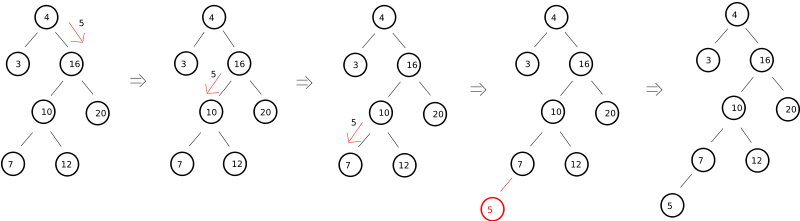
\includegraphics[scale=.45]{7arbolInsercion.jpg}
  \caption{Insercion en árbol}
  \label{fig:7insercion}
\end{figure}

\subsection{Eliminación}
\label{sec:eliminacion}

La operación de borrado no es tan sencilla como las de búsqueda e
inserción. Existen varios casos a tener en consideración:
\begin{itemize}
\item Borrar un nodo sin hijos ó nodo hoja: simplemente se borra y se
  establece a nulo el apuntador de su padre.
\item Borrar un nodo con un subárbol hijo: se borra el nodo y se
  asigna su subárbol hijo como subárbol de su padre.
\item Borrar un nodo con dos subárboles hijo: la solución está en
  reemplazar el valor del nodo por el de su predecesor o por el de su
  sucesor en orden y posteriormente borrar este nodo. Su predecesor en
  orden será el nodo más a la derecha de su subárbol izquierdo (mayor
  nodo del subarbol izquierdo), y su sucesor el nodo más a la
  izquierda de su subárbol derecho (menor nodo del subarbol
  derecho). En la siguiente figura se muestra cómo existe la
  posibilidad de realizar cualquiera de ambos reemplazos:
\end{itemize}
\begin{figure}[H]
  \centering
  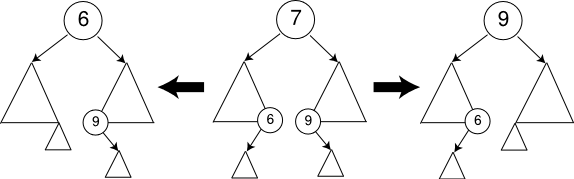
\includegraphics[scale=.55]{8arbolEliminacion.jpg}
  \caption{Eliminación en árbol}
  \label{fig:8arbolEliminacion}
\end{figure}

\begin{verbatim}
class ArbolBinBusqueda:: ArbolBinario {
public:
   ....
   TValor remove(TLlave key) {
      return remove (raiz, key) ;
   }

   TValor remove (NodoBin *n, TLlave key) {
      TValor value = null ;
      NodoBin *padre = null ;

      while (n != nullptr && n->llave != key) {
         padre = n ;
         if (key < n->llave)
            n=n->izq ;
         else
            n = n->der ;
      }

      if (n!=nullptr) {
         value = n->value ;
         if (n->izq == null && n->der == nullptr) { //es nodo hoja
            if (padre->izq == n)
               padre->izq = null ;
            else
                padre->der = null ;
         }else{
            if (n->izq == null) { // sólo tiene hijo derecho
               if (padre->izq == n)
               padre->izq = n->der ;
            else
               padre->der = n->der ;
         }else{
            if (n->der == nullptr) { // sólo tiene hijo izquierdo
               if (padre->izq == n)
                  padre->izq = n->izq ;
               else
                  padre->der = n->izq ;
         }else{ // tiene dos subárboles
            // predecesor en orden
            NodoBin *temp = n->izq ;
            while (temp->der != nullptr)
               temp = temp->der ;
            n->llave = temp->llave ;
            n->valor = temp->valor ;
            remove (n->izq, n->llave) ;
         }//if interno
      }//if
      return value ;
   }//funcion remove
}
\end{verbatim}

En el caso ideal una búsqueda de una llave tiene un orden $O(n)=lg (n)$,
sin embargo puede suceder el fenómeno del desbalance

\subsection{Árbol AVL}
\label{sec:arbol-avl}

El árbol AVL toma su nombre de las iniciales de los apellidos de sus
inventores, Adelson-Velskii y Landis. Lo dieron a conocer en la
publicación de un artículo en 1962: <<An algorithm for the organization
of information>> (<<Un algoritmo para la organización de la
información>>).

Los árboles AVL están siempre equilibrados de tal modo que para todos
los nodos, la altura de la rama izquierda no difiere en más de una
unidad de la altura de la rama derecha. Gracias a esta forma de
equilibrio (o balanceo), la complejidad de una búsqueda en uno de
estos árboles se mantiene siempre en orden de complejidad O(lg n). El
factor de equilibrio puede ser almacenado directamente en cada nodo o
ser computado a partir de las alturas de los subárboles.

Para conseguir esta propiedad de equilibrio, la inserción y el borrado
de los nodos se ha de realizar de una forma especial. Si al realizar
una operación de inserción o borrado se rompe la condición de
equilibrio, hay que realizar una serie de rotaciones de los nodos.

Los árboles AVL más profundos son los árboles de Fibonacci.

\subsubsection{Definición.}
\label{sec:definicion}
\begin{definicion}
  \textbf{Altura de un árbol}.  Sea T un árbol binario de búsqueda y sean Ti y
  Td sus subárboles, su altura H(T), es:
  \begin{itemize}
  \item 0 si el árbol T está vacío
  \item 1 + max(H(Ti),H(Td)) si no está vacío
  \end{itemize}
\end{definicion}

\begin{definicion}
  \textbf{Árbol AVL}.  Sea T un árbol binario de búsqueda (ABB) con Ti
  y Td siendo sus subárboles izquierdo y derecho respectivamente,
  tenemos que:
  \begin{itemize}
  \item Si T es vacío, es un árbol AVL
  \item Si T es un ABB no vacío, es AVL si (si y sólo si):
    \begin{itemize}
    \item[*] Ti y Td son AVL y
    \item[*] -1 <= H(Ti) - H(Td) <= 1
    \end{itemize}
  \end{itemize}
\end{definicion}

Ej: árbol binario de búsqueda desbalanceado
\begin{figure}[H]
  \centering
  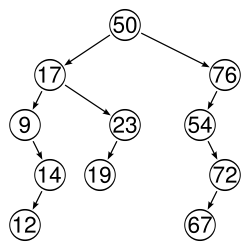
\includegraphics[scale=0.5]{9arbolBinBusquedaDesbalanceado.jpg}
  \caption{Árbol binario de búsqueda desbalanceado}
  \label{fig:9arbolBinBusquedaDesbalanceado.jpg}
\end{figure}

Mismo árbol balanceado
\begin{figure}[H]
  \centering
  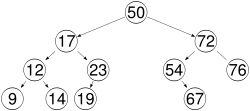
\includegraphics[scale=0.5]{10arbolBinBusquedaBalanceado.jpg}
  \caption{Árbol binario de búsqueda balanceado}
  \label{fig:10arbolBinBusquedaBalanceado}
\end{figure}
Por esta definición tenemos que el árbol de la figura de arriba no es
AVL, mientras que el de abajo sí lo es. Véase también que se trata de
un árbol ordenado, en el cual para cada nodo todos los nodos de su
subárbol izquierdo tienen un valor de clave menor y todos los nodos de
su subárbol derecho tienen un valor de clave mayor que el suyo,
cumpliendo así la propiedad de los ABB.

\subsubsection{Factor de equilibrio}
\label{sec:factor-de-equilibrio}

Cada nodo, además de la información que se pretende almacenar, debe
tener los dos apuntadores a los árboles derecho e izquierdo, igual que
los árboles binarios de búsqueda (ABB), y además el dato que controla
el factor de equilibrio.

El factor de equilibrio es la diferencia entre las alturas del árbol
derecho y el izquierdo:

FE = altura subárbol derecho - altura subárbol izquierdo;

Por definición, para un árbol AVL, este valor debe ser -1, 0 ó 1.

\subsubsection{Operaciones}
\label{sec:operaciones}

Las operaciones básicas de un árbol AVL implican generalmente el
realizar los mismos algoritmos que serían realizados en un árbol
binario de búsqueda desequilibrado, pero precedido o seguido por una o
más de las llamadas <<rotaciones AVL>>.

\paragraph{Búsqueda}
\label{sec:busqueda-1}

Las búsquedas se realizan de la misma manera que en los ABB, pero al
estar el árbol equilibrado la complejidad de la búsqueda nunca
excederá de O(log n).

\begin{verbatim}
class NodoAVL::NodoBin {
   int balance ;
   NodoAVL(TLlave llv, TValor value):NodoBin (llv,value) {
      balance = 0 ;
   }

   NodoAVL *rotacionDer() {
      NodoAVL *temp = izq ;
      izq = izq.der ;
      temp.der = this ;
      return temp ;
   }
}

class ArbolAVL::ArbolBinarioBusqueda {
   private:
      NodoAVL<K,V> raiz ;
   public:
      .....
      TValor get(TLlave llv) {
         NodoBin *temp = raiz ;
         while (temp != nullptr && llv != temp->llv) {
            if (llv < temp>llv) {
               temp = temp.izq ;
            }else{
               temp = temp.der ;
            }
         }
         if (temp == nullptr)
            return nullptr ; // no está
         else
            return temp.valor ;
      }
      .....
}
\end{verbatim}

\paragraph{Inserción}
\label{sec:insercion-1}

La inserción en un árbol de AVL puede ser realizada insertando el
valor dado en el árbol como si fuera un árbol de búsqueda binario
desequilibrado y después retrocediendo hacia la raíz, rotando sobre
cualquier nodo que pueda haberse desequilibrado durante la inserción.

Dado que como mucho un nodo es rotado 1.5 veces log n en la vuelta
hacia la raíz, y cada rotación AVL tarda el mismo tiempo, el proceso
de inserción tarda un tiempo total de O(log n).

\begin{verbatim}
class ArbolAVL::ArbolBinarioBusqueda {
   private:
      NodoAVL *raiz ;
   public:
   .....
   TValor put (TLlave llv, TValor value) {
      bool crecio= false ;
      if (raiz == nullptr) // árbol vacío
         raiz = new NodoAVL(llv, value) ;
      else
         raiz = put(llv, value, raiz, crecio) ;
      return value ;
   }
   NodoAVL *put (TLlave llv, TValor value, NodoAVL *n, bool &crecio) {
      if (llv == n->llv) // ya está ==> error
         throw "Duplicado" ;
      else if (llv < n->llv) { // debe insertarse a la izquierda
         if (n->izq != null) {  // existe hijo izquierdo
            put (llv, value, n->izq, crecio) ;
            if ( crecio ) {
               n->balance -- ;
               if (n->balance < -1) { //necesario balancear
                  if ( n->izq->balance > 0 ) //rotación doble
                     n->izq = n->izq->rotacionIzq() ;
                  crecio = false ;
                  return n->rotacionIzq() ;
               }
            }
         }else{ // no existe hijo izquierdo
            n->izq = new NodoAVL(llv, value) ;
            n.balance -- ;
            crecio = (n.balance!=0) ;
         }
      }else{  // debe insertarse en la derecha
         if (n->der != nullptr) { // existe hijo derecho
            put (llv, value, n->der, crecio) ;
            if ( crecio ) {
               n->balance ++ ;
               if (n->balance > 1) { //necesario balancear
                  if ( n->der->balance < 0 ) //rotación doble
                     n->der = n->der->rotacionDer() ;
                  crecio = false ;
                  return n->rotacionIzq() ;
               }
            }
         }else { //no existe hijo derecho
            n->der = new NodoAVL(llv, value) ;
            n.balance ++ ;
            crecio = (n->balance!=0) ;
         }
     }
} 
\end{verbatim}

\paragraph{ Extracción}
\label{sec:extraccion}

El problema de la extracción puede resolverse en O(log n) pasos. Una
extracción trae consigo una disminución de la altura de la rama donde
se extrajo y tendrá como efecto un cambio en el factor de equilibrio
del nodo padre de la rama en cuestión, pudiendo necesitarse una
rotación.

Esta disminución de la altura y la corrección de los factores de
equilibrio con sus posibles rotaciones asociadas pueden propagarse
hasta la raíz.

\subsection{Árbol HB[K]}
\label{sec:arbol-hbk}
Sea T un árbol binario de búsqueda (ABB) con Ti y Td siendo sus
subárboles izquierdo y derecho respectivamente, tenemos que:


Si T es vacío, es un árbol HB[k]

Si T es un ABB no vacío, es HB[k] si y sólo si:

\begin{itemize}
\item Ti y Td son HB[k] y
\item -k <= H(Ti) - H(Td) <= k
\end{itemize}

\textbf{HB[1] = AVL }

\section{Árboles B}
\label{sec:arboles-b}

Hasta ahora se ha descrito sólo árboles binarios. Sin embargo, en las
aplicaciones donde se necesitan árboles de búsqueda a gran escala son
necesarios los árboles multicaminos, o multihijos. Éstos tienen la
propiedad que pueden tener más de un hijo por nodo.

Un árbol B de orden k (k>=2), tiene las siguientes propiedades:

\begin{enumerate}
\item Es un árbol de búsqueda
\item Todos los nodos tienen como máximo de $k$ llaves
\item Todos los nodos tienen como mínimo el piso $(k/2)$ llaves,
  excepto la raíz que puede tener 1
\item Un nodo con $x$ llaves tiene $x+1$ hijos o es hoja
\item Todas las hojas aparecen en el mismo nivel
\end{enumerate}

\section{Ejercicios}
\label{sec:ejercicios}

\subsection{Árboles HB[K]}
\label{sec:arboles-hbk}

Dadas las siguientes clases:

\begin{verbatim}
template <class T>
class NodoBin {
public:
    T valor ;
    NodoBin *izq ;
    NodoBin *der ;


    NodoBin();
    virtual ~NodoBin();
};

template <class T, class K>
class NodoBinBusq: NodoBin<T> {
public:
    K llave ;


    NodoBinBusq();
    virtual ~NodoBinBusq();
};

template <class T, class K>
class ArbolBinBusq {
public:
    ArbolBinBusq();
    virtual ~ArbolBinBusq();

    //* retorna true si el árbol es un HB[k], caso contrario retorna false

    bool esHB(int k) ;

    //* retorna la alturna del árbol

    int altura() ;

private:

     NodoBinBusq *raiz;

.....

};
\end{verbatim}
Implementar los métodos ArbolBinBusq::altura() y
ArbolBinBusq::esHB(int k).  Este último debe ser O (n)=n.

No utilizar ninguna estructura de datos adicional.

Entregar compilables: .h y .cpp

\subsection{Árbol en arreglo}
\label{sec:arbol-en-arreglo}

Dado un árbol binario de búsqueda, representado en un arreglo
unidimensional, haga un algoritmo que realice un recorrido tal que
imprima las llaves en orden descendente.  No utilizar ninguna
estructura de datos adicional.  El orden debe ser O(n)=n

\subsection{Árbol de expresiones}
\label{sec:arbol-de-expresiones}

Dada una clase ArbolExp, que representa un árbol de expresiones,
escriba un método valor() que dé como resultado el valor de la
expresión representada. Puede suponer que sólo existen los operadores
de suma, resta, multiplicación y división. También se supone que todos
los operandos son constantes, es decir no hay variables. No debe
utilizar ninguna estructura de datos adicional. Suponga que sólo
existen las siguientes variables de cada clase:

\begin{verbatim}
class ArbolExp {

public:

......

int valor ( ) ;

....

private:

NodoExp *raíz ;

….

}


class NodoExp {

…..

void *valor ; //constante u operador

NodoExp *izq ;

NodoExp *der ;

……

}
\end{verbatim}

\subsection{Ordenamiento de árbol B[k]}
\label{sec:orden-de-arbol}

Escriba un método de una clase ArbolB, que representa un árbol B[k],
que imprima las llaves en orden de mayor a menor. Dicho algoritmo debe
ser de orden O(n)=n y no debe utilizar ninguna estructura de datos
adicional. Suponga que sólo existen las siguientes variables de cada
clase:

\begin{verbatim}
class ArbolB {

public:

......

void recorridoInverso() ;

....

private:

NodoB *raíz ;

int k ;

….

}

class NodoB {

…..

int llaves[] ;

int info[];

NodoB* hijo[]

int k ;

int numElementos ;

……

}
\end{verbatim}

%%% Local Variables:
%%% TeX-master: "tedd"
%%% End:



\chapter{Tablas de dispersión}

En esta unidad revisaremos otra estructura para uso de contenedores,
que busca obtener el rendimiento de los arreglos lexicográficos y
la flexibilidad en el uso de memoria de los árboles. El contenido
básico es:

  \begin{itemize}
  \item Componentes generales de una tabla de dispersión
  \item Compresión
  \item Funciones de dispersión
  \item Resolución de colisiones
  \end{itemize}

\section{Componentes generales de las tablas de dispersión}
\label{sec:comp-gener-de}

Hemos visto, como estructura de contenedor, los arreglos y los
árboles, cada uno con sus propias ventajas y desventajas.  Por un lado
los arreglos lexicográficos con una gran eficiencia de acceso, y
por otro, los árboles con el dinamismo y optimización en el uso de la
memoria.  ¿Y si pudieramos tener una estructura que combine las
ventajas de los arreglos lexicográficos y árboles?

Esa es la idea principal de los proponentes de las tablas de
dispersión, por un lado se tiene una tabla representada en una arreglo
lexicográfico, que puede tener elementos dinámicos para crecimiento a
futuro.

Los componentes general de una tabla de dispersión se resumen en la
siguiente gráfica.

\begin{center}
  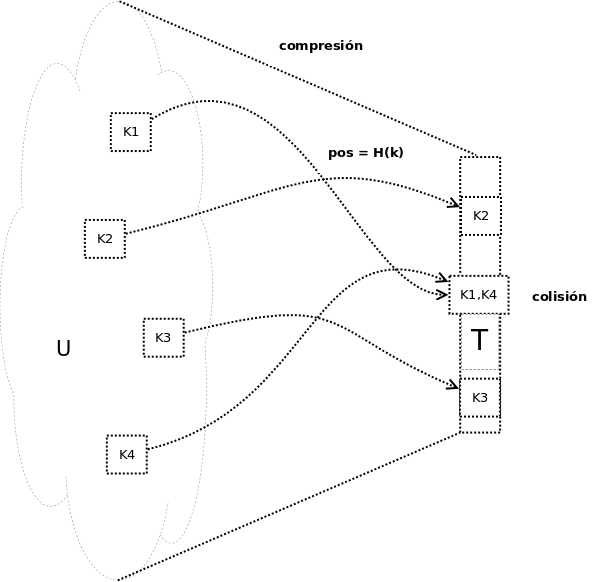
\includegraphics[scale=.35]{1.png}
\end{center}

Podemos distinguir los siguientes elementos:

\begin{itemize}
\item Hay un universo U de elementos posibles que pueden llegar a ser
  utilizados en la memoria
\item Tenemos la tabla T, que es un arreglo lexicográfico en la
  memoria de la computadora, con los elementos de U, realmente
  utilizados
\item Los elementos de U están identificados por llaves $k_i$
\item Las llaves de cada elemento son mapeadas a posiciones
  individuales por medio de una función de dispersión ( \textbf{pos =
    h(k)} )
\item Dado que las llaves $k_i$ pueden ser alfanuméricas, puede existir
  primero una conversión de alfanumérico a numérico.  Este proceso de
  conversión y mapeo puede ser considerado dentro de la misma función
  de dispersión \textbf{h(k)}
\item Dado que \textbf{U $>>$ T} (hay muchos más elementos en \textbf{U}
  que en \textbf{T}) invariablemente se dará el caso en que dos llaves
  mapearán a la misma posición.  Ésto es una \textbf{colisión}.
\end{itemize}

\section{Políticas de resolución de colisiones}
\label{sec:polit-de-resol}

Además de la función de dispersión H(K), el otro componente de las
tablas de dispersión es la política de resolución de colisiones.

Esta política se refiere a la estrategia que se usará para resolver el
problema de las colisiones, que inevitablemente se dará, dado el hecho
que el número de elementos posible en el universo, es mucho mayor que
el número de elementos que caben en la tabla en memoria.

La elección de la política de resolución es tan importante que
normalmente esta decisión da nombre a la estructura, como veremos en
las siguientes secciones.  

\section{Dispersión por encadenamiento}
\label{sec:disp-por-encad}

La forma más simple, es que cada posición de la tabla tiene un
apuntador a una lista que contiene todos los elementos que
colisionaron en esa posición, así:

Esta estrategia tiene la ventaja que es relativamente simple de
implementar, sin embargo su rendimiento, O(n), varía entre
\textbf{n/m} y \textbf{n}. Donde \textbf{n} es el número de elementos
en la tabla y \textbf{m}.

El rendimiento está dado así porque, en el mejor de los casos, en que
la función de dispersión cumple con repartir uniformente los elementos
en la tabla, las listas en cada posición, en el largo plazo, tendrán
la misma cantidad de elementos (\textbf{n/m}).  El acceso a una
posición de la tabla está dado por la ejecución de H(k), lo que se
toma como O(n)=1, y la búsqueda en una lista esta dado por el tamaño
de la lista, por lo tanto O(Tabla.get(k)) = n/m.

Sólo en el caso extremo, en que todos los elementos colisionen en la
misma posición, el rendimiento se degenerará a O(n)=n, dado que todos
los elementos de la tabla estarán en la misma lista.

En busca de optimizar dicho rendimiento, se ha pensado en utilizar
árboles AVL en vez de listas.  Esto implica que O(n) = lg (n/m).  Otra
vez, debido a que los árboles tenderán a tener la misma cantidad de
elementos: n/m.

De forma similar, si usaramos árboles B[k], tendríamos un rendimiento
O(n) = logk(n/m).

En general, cualquier estructura dinámica que se use para resolver la
colisión, el efecto es que el rendimiento se multiplicará, dado que es
más eficiente buscar en una lista o árbol de tamaño \textbf{n/m} que
en una lista o árbol de \textbf{n}, si no usaramos una tabla de
dispersión.

\section{Direccionamiento abierto}
\label{sec:direcc-abierto}

Al contrario del encadenamiento, no utiliza memoria adicional a la
tabla en sí.  Las colisiones se resuelven dentro de la misma tabla,
así:

\begin{center}
  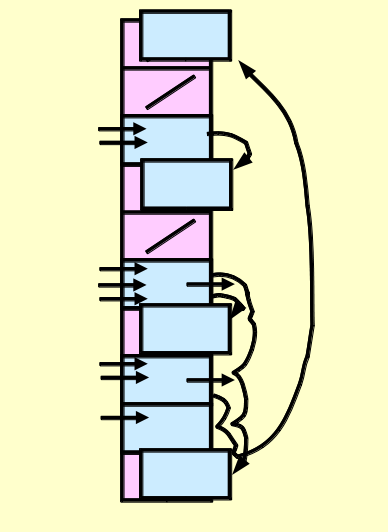
\includegraphics[scale=.5]{3.png}
\end{center}

Básicamente, cuando una llave colisiona en una posición, se sigue la
siguiente estrategia:
\begin{itemize}
\item Se realiza un ciclo de intentos de buscar una posición al elemento
  \begin{itemize}
  \item En cada intento se examina la posición dada por
    \textit{posición actual + S(k,i) \% m} , donde \textit{k} es la
    llave a insertar, \textit{i} es el número de intento y
    \textit{S(k,i)} es la función que determina la \textbf{secuencia
      de prueba}.
  \item Si la posición examinada esta libre, entonces se asigna dicha
    posición y se finaliza
  \end{itemize}
\end{itemize}
    
Según la naturaleza de \textit{S(k,i)}, puede ser que los intentos
generen un ciclo infinito de intentos, por lo que debe establecer un
límite al número de intentos. Dicho límite establecerá el rendimiento
máximo de la estructura.  Diferentes autores han propuesto diferentes
límites, que van desde \textit{m/e} hasta \textit{2m}, donde e es la
constante de Euler.  Esto dependerá del diseñador de la estructura.

\textit{S(k,i)} determinará el comportamiento de la política, que
puede ser:
        
\begin{description}
\item[Lineal: ] \textit{S(k,i)=1}, lo que significa que se examinarán
  posiciones continuas a la posición de colisión.  Ésto provocará que
  se formen grupos de llaves continuas que irán creciendo conforme se
  inserten más llaves.  Ésto se denomina agrupamiento primario.
\item[Cuadrática: ] $S(k,i)=i^2$ creará secuencias de pruebas con saltos
  de la forma 1, 4, 9, 16,.... a partir de la posición de colisión.
  Ésto elimina el agrupamiento primario, pero provoca que todas las
  llaves que colisionan en una misma posición, sigan la misma
  secuencia de prueba, lo que se denomina agrupamiento secundario.
\item[Doble dispersión: ] \textit{S(k,i)= ( k \% c +1 ) * i}.  Se
  utiliza una segunda función de dispersión (por ejemplo \textit{k \%
    c +1} ) lo cual agrega una variación de una llave a otra, por lo
  que, aunque dos llaves colisionen en la misma posición, seguirán
  secuencias de prueba distintas.
\end{description}

\begin{center}
  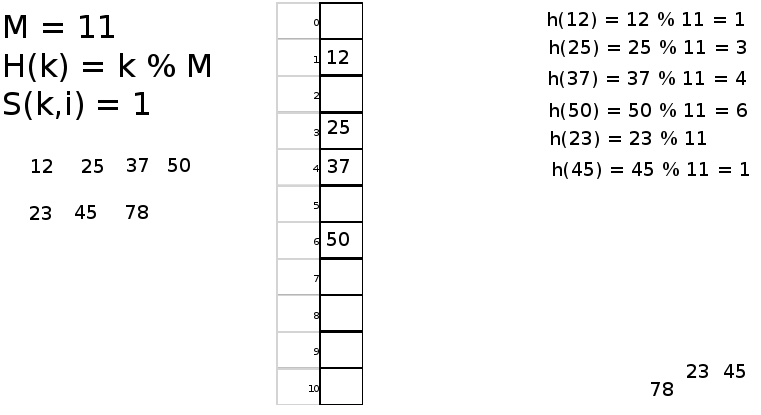
\includegraphics[scale=.4]{4.png}
\end{center}

\begin{center}
  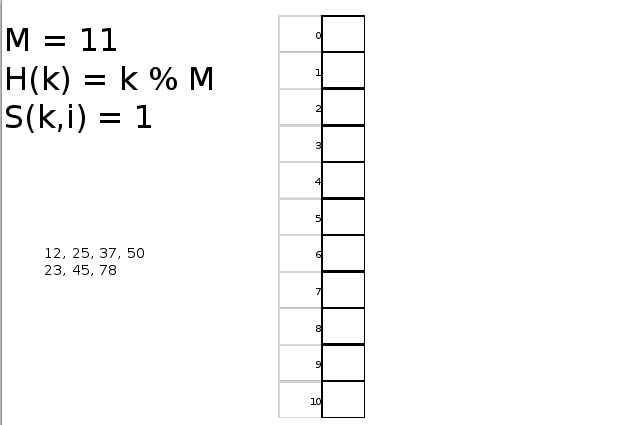
\includegraphics[scale=.4]{5.png}
\end{center}

%%% Local Variables:
%%% TeX-master: "cdc"
%%% End:


\chapter{Textos}
\label{cha:textos}
Estudio de las diferentes representaciones y aplicaciones del manejo
de textos o strings.
\section{Generalidades}
Los textos son, por mucho, las estructuras de datos más utilizadas en
la computación.  Toda operación en una computadora implica algún
procesamiento de texto.  Por ejemplo:

\begin{itemize}
\item Compilar un programa: significa procesar un texto de entrada,
  que es el programa fuente, hecho en algún lenguaje de programación
  legible para los humanos, para producir un texto de salida: un
  programa binario, que legible para la computadora, que aunque el
  humano no lo puede leer directamente, sigue siendo un texto
\item Procesador de palabras: lee del teclado, letras y comandos que
  generarán un texto.  En estos programas usualmente hay muchas
  operaciones adicionales sobre los textos como la verificación de
  ortografía, formateo de la impresión, etc.
\end{itemize}

En general, los textos se utilizan en todos las aplicaciones que
exista comunicación entre dispositivos, entre computadoras, entre
computadoras y personas.

Claro que cuando hablamos de textos como estructura de datos, ya no
estamos hablando de contenedores mapas, como árboles y tablas, ya que
no hay elementos de un mismo tipo que se puedan acceder por una llave.

Los textos son estructuras de datos, ya que se trata de conjuntos de
datos semánticamente relacionados, con la cual se pueden realizar
distintas operaciones y transformaciones.  También existen diferentes
formas de representación que influirán en el desempeño de una
aplicación.

\begin{quote}
  \textbf{Texto}

  Secuencia de caracteres de longitud finita, que se usa para
  representar información semánticamente relacionada.
\end{quote}

Nótese que esta definición acepta desde los textos legibles por
humanos, programas ejecutables y paquetes de transmisión en la red.

\subsection{Representaciones}
\label{sec:representaciones}

Normalmente estamos acostumbrados a una sólo representación de textos,
que es la representación contigua con \textbf{codificación de longitud
  fija}, como la codificación ASCII o la UNICODE.  Sin embargo veremos
que existen otras codificaciones, no necesariamente contiguas y donde
el número de bits utilizado para representar cada caracter puede
variar de caracter a caracter.

\subsection{Operaciones}
\label{sec:operaciones}

Cuando se habla de operaciones sobre textos o strings, inmediatamente
pensamos en catenación, eliminación de caracteres o inserción de
caracteres.  Sin embargo éstas no son las únicas operaciones que
podemos hacer en un texto, y, sin darnos cuenta, las realizamos en
muchas aplicaciones de la vida diaria.

Las operaciones que vamos a estudiar son:

\begin{description}
\item[Encriptación: ] Transformación de un texto legible en uno
  ilegíble (criptograma) que sólo puede ser interpretado por quien
  tenga una palabra oculta (contraseña)
\item[Búsqueda de patrones: ] Consiste en buscar dentro de texto si
  existe o no una palabra determinada (patrón) y, si existe,
  determinar la posición o posiciones donde se encuentra.
\item[Macroexpansión: ] Consiste en expandir un abreviatura de un
  texto, a otro texto basado en parámetros. Por ejemplo: lo que
  realiza el precompilador de C/C++ con las directivas \#define.
\item[Compresión: ] Es la transformación que consiste en representar
  un texto en menos espacio que en su representación normal.
\end{description}

\section{Búsqueda de patrones}
\label{sec:busqueda-de-patrones}

La búsqueda de patrones es una de las operaciones más comunes a
realizar en los textos en cualquier aplicación.

La operación básica es que se tiene un texto de $n$ caracteres $S[n]$
y un texto de $m$ caracteres $p[m]$, donde $m \leq n$, y se desea
determinar si $p[m]$ forma parte de $s[n]$, y si es así determinar la
posición dentro de $s[n]$ donde se encuentra.

Existen diferentes métodos para realizar esta operación:
\begin{itemize}
\item Búsqueda simple o de fuerza bruta
\item Booyer Moore
\item Knutt Morris Pratt
\end{itemize}
Las cuales detallaremos a continuación.

\subsection{Búsqueda simple o de fuerza bruta}
\label{sec:busqueda-simple-o}

Es el método en el cual se compara directamente caracter a caracter
cada una de las posiciones de $p[m]$ en $s[n]$.  Se puede realizar con
el siguiente algoritmo:

\begin{verbatim}
int buscar (char *p, char *s, int m, int n) {
    while (i <= n-m && !encontrado)
    {          
        j = 1 ;
        while (j <= m && i+j-1<=n && s[i+j-1] == p[j])
            j ++ ;
        i ++ ;
        encontrado = (j > m) ;
    }

    return encontrado?i:-1 ;
}
\end{verbatim}

Si vemos el proceso como una sucesión de superposiciones de s[n] y
p[m], la ejecución del algoritmo, sobre s[10]=''HOLALALASA'' y
p[5]=''LALAS'' puede verse así:

\begin{verbatim}
\end{verbatim}

\begin{alltt}
  H O L A L A L A S A

  {\bf L} A L A S

  {\bf L} A L A S

  {\bf L A L A S}

  {\bf L} A L A S

  {\bf L} A L A S <---- encontrado
\end{alltt}

La letra negrilla indica el caracter de p[m] que se compara con la
posición superpuesta de s[n] y el subrayado indica la comparación que
falla.

El rendimiento de éste algoritmo es de \textbf{n*m} ya que en el peor
de los casos se compararán todas las posiciones de p contra s, por
ejemplo: si s[9]=''LALALALAS'' y p[3]=''LAS''

Ejercicio: demostrar que el O(buscar(n,m)) = n*m

\subsection{Boyer Moore y Knutt Morris Pratt}
\label{sec:boyer-moore-y}
\href{http://users.dcc.uchile.cl/~bebustos/apuntes/cc30a/BusqTexto/}{Búsqueda
  en texto.}

\section{Encripción}
\label{sec:encripcion}

La encripción es una operación sobre textos que consiste en una
transformación de un texto legible, para transformarlo en un texto
ilegible, que pueda ser transmitido por un medio público sin que pueda
ser descifrado, sino hasta que llegue al destinatario, quien podrá
aplicar la transformación inversa y obtener el texto original.

Este proceso se ilustra en la siguiente gráfica:

\begin{center}
  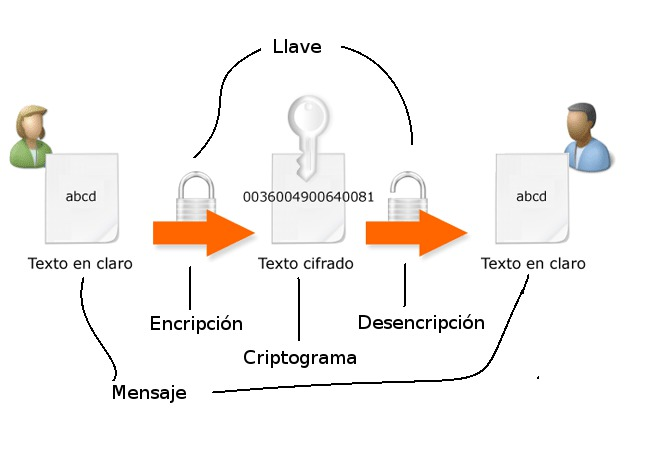
\includegraphics[scale=.7]{1textos.jpg}
\end{center}

Como podemos apreciar, hay varios elementos involucrados:
\begin{description}
\item[Mensaje: ] Es el texto legible para cualquier persona
\item[Llave: ] Es una palabra o contraseña secreta, que sólo sabe el
  remitente y el destinatario del mensaje
\item[Encripción: ] Es la operación de transformar el texto en claro,
  utilizando la llave, en un texto ilegible
\item[Criptograma: ] es el texto ilegible, resultado de la operación
  de encripción
\item[Desencripción: ] Es la operación de transformar el criptograma
  en el texto original, utilizando la llave predeterminada.
\end{description}

Mas formalmente podemos decir que la encripción es:

\begin{quote}
  Si se tiene un texto T y una clave K, se puede aplicar una función
  de encripción E(T,K) = C, donde C se llama criptograma, al cual se
  le puede aplicar una función de desencripción D(C,K) = T para
  obtener el texto original
\end{quote}

El uso de la encripción viene desde los inicios de la historia, desde
que las personas han deseado la privacidad, pero la aplicación
principal ha sido la guerra.

Los espartanos, son de los primeros que se sabe hacían uso de la
encripción en el Siglo V AC, empleando cintas de lino y un bastón
llamado escitalo. La cinta se enrollaba en el bastón y se escribía el
texto transversalmente en el bastón, tal como se muestra en la
siguiente gráfica:

\begin{center}
  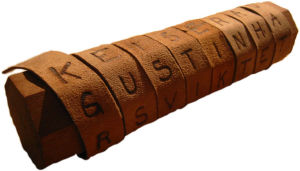
\includegraphics{2textos.jpeg}
\end{center}

El mensajero se le entregaba la cinta, la cual al extenderla era
ilegible.  Para descifrarla, el destinatario debería tener un bastón
del mismo diametro, enrollar la cinta, y leer la sección transversal
que tuviera sentido.  Este tipo de encripción es lo que actualmente se
llama \textbf{transposición}, porque se cambia de sitio los símbolos
del mensaje original

En Roman, Julio César desarrolló un mecanismo de codificación que
lleva su nombre.  Consiste en la \textbf{sustitución} de cada letra
por la que aparece tres posiciones a su derecha en el alfabeto, así la
A se convierte en D, la B en E y así sucesivamente.  Ejemplo:

\begin{quote}
  JUAN -> KVBO (corrimiento de 1 caracter)
\end{quote}

Otro método más moderno es la \textbf{confusión} u
\textbf{ofuscación}, que consiste en ocultar mensajes dentro de otro
mensaje claro.  Ejemplo de ésto es lo que comunmente se llama ''leer
entre líneas''.  Por ejemplo:

\begin{alltt}
  Éste es un mensaje

  en el cual no hay nada

  oculto entre

  este mensaje y

  otro mensaje que

  aunque es peligroso

  parece inofensivo

  y puede representar

  ante los que no sepan leer

  la sabiduría que está

  entre líneas.
\end{alltt}

Leer este mensaje de forma normal no releva nada claro, pero si leemos
las líneas impares podremos leer el mensaje ''\textit{Éste es un
  mensaje oculto entre otro mensaje que parece inofensivo ante los que
  no sepan leer entre líneas}''.

La \textbf{estenografía}, aunque algunos autores no la consideran
encripción en sí, es un método que aprovecha los vacíos que se dan
entre los diferentes formatos de gráficos y multimedios para ocultar
información.  Por ejemplo en el formato jpg hay espacios que no se
utilizan como parte de la gráfica que representa, por lo tanto, dichos
espacios pueden ser utilizado para poner información.  Lo mismo sucede
con el formato \textbf{mp3}, y otros formatos de música y gráficos.

Claro que en la computación moderna, éstos métodos distan mucho de ser
efectivos, ya que serían fácilmente descifrados.  Actualmente se han
desarrollado una gran cantidad de algoritmos y métodos de encripción,
los cuales clasificaremos en dos grupos:

\begin{enumerate}
\item encripción simétrica o privada
\item Encripción asimétrica o pública
\end{enumerate}

\subsection{Encripción simétrica o privada}
\label{sec:encr-simetr-o}

Es el primer tipo de encripción moderno trabajado a nivel
computacional, incluyen máquinas como la máquina codificadora
\textbf{Enigma}, durante la Segunda Guerra Mundial, en el cual la
misma llave utilizada para encriptar, es la que se necesita para
realizar la desencripción. Un ejemplo simple es la mezcla con
secuencias fijas aleatorias, en la cual se aprovecha la siguiente
propiedad de la operación xor

sea x \& y dos enteros independientes, entonces se cumple que
\begin{itemize}
\item (x xor y) xor x = y
\item (x xor y) xor y = x
\end{itemize}

Si T es el texto a encriptar, T se ve como una secuencia de enteros
$T_1T_2T_3...T_n$.  La llave secreta K, también se ve como una
secuencia de enteros $K_1K_2K_3...K_m$, donde m $\leq$ n.  El
criptograma C, visto como $C_1C_2C_3...C_n$ se forma por sucesivas
operaciones xor, de superposiciones de la llave K sobre el texto T,
así:

\[
\begin{array}{|cccccccccc|}
  \hline
  T   & T_1 & T_2 & ... & T_m & T_{m+1} & T_{m+2} & ... & T_{n-1} & T_n \\ 
  &    &    &     &  xor &      &      &     &      &      \\
  K   & K_1 & K_2 & ... & K_m & K_1   & K_2   & ... & K_i   & K_{i+1} \\
  &    &    &     &  =   &      &      &     &      &      \\
  C   & C_1 & C_2 & ... & C_fm & C_{m+1} & C_{m+2} & ... & C_{n-1} & C_n \\
  \hline
\end{array}
\]

y la operación de desencripción sería así:

\[
\begin{array}{|cccccccccc|}
\hline
  C   & C_1 & C_2 & ... & C_m & C_{m+1} & C_{m+2} & ... & C_{n-1} & C_n\\
       &    &    &     &    & xor     &      &     &      &      \\
  K   & K_1 & K_2 & ... & K_m & K_1   & K_2   & ... & K_i   & K_{i+1}\\
      &    &    &     &    &  =    &      &     &      &      \\
  T   & T_1 & T_2 & ... & T_m & T_{m+1} & T_{m+2} & ... & T_{n-1} & T_n\\
\hline
\end{array}
\]

Una encripción simple y eficiente, pero en una combinatoria de $16^m$
puede encontrarse la llave K (suponiendo que 16 bits es el tamaño de
un entero).

Entre los algoritmos de encripción simétrica actuales se encuentran:

\begin{itemize}
\item DES (Data Encryption Standard): llave de 56 bits de longitud,
  tiempo menor a 3 meses para desencriptar el mensaje
\item Triple – DES
\item Advanced Encryption Standard  (AES)
\item Blowfish
\end{itemize}
    
A pesar de la importancia que han tenido (y seguirán teniendo) la
encripción simétrica, en nuestro mundo actual de comunicación masiva y
globalizada, tener comunicación privada, a través de estos métodos,
presentan dos problemas importantes:

\begin{description}
\item[La paradoja del canal seguro: ] si deseamos encriptar un
  mensaje, es porque seguramente debemos enviarlo a través de un medio
  o canal que se considera inseguro, como el correo electrónico.  El
  problema se deriva que el destinatario está geográficamente distante
  y no es posible enviarla la contraseña por un medio seguro, y si
  hubiera un medio seguro, no sería necesario encriptar el mensaje
\item[La multiplicidad de intercambios: ] Si 2 personas necesitan
  comunicación privada, deben realizar un intercambio de llaves.  Si
  son 3 personas, deben realizar un total de 6 intercambios (2 por
  cada participante), sin son 4, 12 intercambios y así sucesivamente,
  que resulta en que si \textbf{n} personas desean comunicarse
  privadamente, deben haber \textbf{n*(n-1)} intercambios, lo que
  representa un órden cuadrático.
\end{description}

Estos problemas hicieron que la encripción simétrica fuera
insuficiente para lograr una comunicación privada eficiente en el
Internet, y es allí donde cobra importancia la encripción asimétrica.

\subsection{Encripción asimétrica o pública}
\label{sec:encr-asim-o}

El RSA es el criptosistema de llave pública más popular basado en el
modelo de Diffie-Hellman, el cual ofrece encripción y firmas digitales
(autentificación). Ron Rivest, Adl Shamir y Leonard Adleman
desarrollaron el RSA en 1977, de ahí su nombre formado por la primera
letra del apellido de sus inventores.

La base de este sistema es la compleja matemática detras de la
factorización de números primos grandes (ver links publicados), que
van desde 128 bits hasta 1024, lo cual está fuera del alcance del
curso.  Sin embargo, lo importante de este método es que tiene las
siguientes propiedades:

\begin{enumerate}
\item Cada usuario tiene dos llaves, una privada y otra pública.  La
  llave privada es conocida sólo por el propietario y normalmente es
  almacenada en un archivo protegido por una llave simétrica, conocida
  sólo por el dueño.  La llave pública, por el contrario debe ser
  conocida por todos los posibles destinatarios, y generalmente se
  publica por cualquier canal inseguro (correo electrónico, redes
  sociales, directorio públicos, etc)
\item Sea
  \begin{enumerate}
  \item T el texto o mensaje en claro
  \item $X_{prv}$ la llave privada de la persona X
  \item $X_{pbl}$ la llave pública de X
  \item C=E(T,K) la función de encripción del texto T con la llave K,
    que da como resultado el criptograma C
  \item T=D(C, K) la función de desencripción del criptograma C, con
    la llave K, que da como resultado el texto T
  \item Entonces, para RSA se cumple que:
    \begin{enumerate}
    \item si C=E(T, $X_{prv}$) entonces T=D(C, $X_{pbl}$), es decir lo que se
      encripta con la llave privada, sólo puede desencriptarse con la
      llave pública
    \item si C=E(T,$X_{pbl}$ entonces T=D(C, $X_{prv}$), es decir los que se
      encripta con la llave pública, sólo puede desencriptase con la
      llave privada
    \end{enumerate}
  \end{enumerate}
\end{enumerate}

Estas propiedades eliminan los problemas de la paradoja del canal
seguro, por el uso de la llave pública, y la multiplicidad de
intercambios, ya que para que n personas se comunican, sólo se
necesitan n intercambios de llaves públicas.

Además ya se puede realizar una comunicación privada así:
\begin{itemize}
\item Si X envía un mensaje a Y, encriptado con $X_{prv}$, Y lo
  desencriptará con $X_{pbl}$, con lo cual Y estará seguro que X es el
  remitente, ya que el mensaje fue encriptado con $X_{prv}$
\item Si X envía un mensaje a Y, encriptado con Ypbl, Y lo
  desencriptará con Yprv, con lo cual X estará seguro que sólo Y podrá
  leerlo, ya que sólo Y conoce Yprv
\item Al combinar ambos mecanismos, X puede crear un criptograma, en
  el cual se X se asegure que sólo Y puede verlo y Y estará seguro que
  X es el remitente, así:
  \begin{itemize}
  \item X encriptará así:
    \begin{itemize}
    \item $C_1$ = E (T, $X_{prv}$)
    \item $C_2$ = E ($C_1$, Ypbl)
    \end{itemize}
  \item Se envía $C_2$ a Y
  \item Y desencriptará así:
    \begin{itemize}
    \item $C_1$= D ($C_2$, Yprv)
    \item T = D ($C_1$, $X_{pbl}$)
    \end{itemize}
  \end{itemize}
\end{itemize}

Estas propiedades han hecho de RSA la base de todos los protocolos de
seguridad que conocemos, como PGP, HTTP, SSL, etc.  Sin embargo,
debido a su complejidad matemática, que involucra operaciones de
exponentes y módulos con número grandes (de hasta 1024 bits o sea
$2^{1024}$), su rendimiento es mucho menor que el de un algoritmo
simétrico.  Por lo tanto, los protocolos mencionados, hacen una
combinación de métodos simétricos y asimétricos, en los que éstos
últimos, se utilizan sólo para intercambiar una llave simétrica
temporal, generada en tiempo de corrida, al principio de la
comunicación y luego la información se intercambia utilizando un
algoritmo simétrico.


De esta forma se logra una privacidad completa, a través de la
asimetría, con un rendimiento aceptable, a través de la simetría.

\subsection{Criptotutorial}
\label{sec:criptotutorial}

\url{http://www.ti89.com/cryptotut/rsa2.htm}

\subsection{RSA Theory}
\label{sec:rsa-theory}
\url{http://www.di-mgt.com.au/rsa_theory.html}


%%% Local Variables:
%%% TeX-master: "tedd"
%%% End:



\chapter{Ejercicios de exámen}
Alguno ejercicios resueltos de exámen. Otros solo se presentan, más
carecen de solución.
\section{Deducción de O(n) 1}
Deduzca formalmente $O(n)$, mostrando claramente su procedimiento,
para la siguente función:

\begin{lstlisting}[style=miEstilo, numbers=none]
int recursiva1(int n)
{
   if(n<=1)
      return 5;
   else
      return recursiva1(n/2) + recursiva1(n/2);
}
\end{lstlisting}

\[ T(recursiva1(n))=T(n)\]
$$$$
\begin{equation*}
  \label{eq:definicion-por-partes1}
  T(n) = \left\{
    \begin{array}{ll}
      \mathrm{si\ } n \le 1 \; :    &  T(comp_{if})+T(return)=2t\\
      &\\
      \mathrm{si\ } n > 1 \; : &  T(comp_{if})+T(return)+T(n/2)+T(n/2)\\
               & =\;t+t+2T(n/2)\\
               & =\;2t+2T(n/2)
    \end{array}
  \right.
\end{equation*}

Expandiendo parte recursiva:
\begin{eqnarray*}
  \label{eq:1}
  T(n)&=&\mathbf{2t}+2\,T(n/2)\\
  &=&2t+2[2t+2T(n/4)]=2t+4t+4T(n/4)=\mathbf{6t}+4\,T(n/4)\\
  &=&6t+4[2t+2T(n/8)]=6t+8t+8T(n/8)=\mathbf{14t}+8\,T(n/8)\\
  &=&14t+8[2t+2T(n/16)]=14t+16t+16T(n/16)=\mathbf{30t}+16\,T(n/16)\\
  &=&30t+16[2t+2T(n/32)]=30t+32t+32T(n/32)=\mathbf{62t}+32\,T(n/32)
\end{eqnarray*}

las partes en negrita de las expansiones puede escribirse tambien como
\begin{eqnarray*}
  2t&=&2t\\
  6t&=&2t+4t\\
  14t&=&2t+4t+8t\\
  30t&=&2t+4t+8t+16t\\
  62t&=&2t+4t+8t+16t+32t
\end{eqnarray*}

y para un k-ésimo término
$$t\,\sum_{x=1}^k2^x$$

dado que para cada número natural $n$, $2^0+2^1+2^2 \ldots +2^n=2^{n+1}-1$, la
enterior sumatoria queda

\begin{eqnarray*}
  t\,\sum_{x=1}^k2^x&=&t(2^0+2^1+2^2 + 2^3 \ldots +2^k \textcolor{green}{-1})\\
  &=&t(2^{k+1}-1 \textcolor{green}{-1})\\
  &=&t(2^{k+1}-2)\\
  &=&t(2^k2-2)\\
  &=&2t(2^k-1)
\end{eqnarray*}

el $\textcolor{green}{-1}$ restado a la ecuacion es para anular el $2^0$ de la secuencia
y así quede igual a la secuencia que es necesaria.

ahora para un k-ésimo término de la funcion $T(n)$ completa sería
\begin{equation}
  \label{eq:2}
  T(n)=2t(2^k-1)+2^k\,T(n/2^k)
\end{equation}

condicion de salida

\begin{eqnarray*}
  \label{eq:3}
  \frac{n}{2^k}&=&1\\
  n&=&2^k\\
  \log_{2}n&=&\log_{2}2^k\\
  k&=&\log_{2}n
\end{eqnarray*}

sustituyendo $k$ en \ref{eq:2} 

\begin{eqnarray*}
  T(n)&=&2t(2^{\log_{2}n}-1)+2^{\log_{2}n}\,T(n/2^{\log_{2}n})\\
  &=&2t(n-1)+n\,T(n/n)\\
  &=&2t(n-1)+n\,T(1)\\
  &=&2t(n-1)+n\,(2t) \;\;\;\;  \setminus \text{usando la parte no recursiva de T(n)}\\
  &=&2t(n-1+n)\\
  &=&2t(2n-1) \;\;\;\;  \setminus \text{por definición, tiempo minimo igual a 1 (t=1)}\\
  &=&4n-2
\end{eqnarray*}

deduciendo O(n)

\begin{eqnarray*}
  O[T(recursiva1(n))]&=&O[4n-2]\\
  &=&max(O(4n), O(-2))\\
  &=&O(4n)\\
  &=&n
\end{eqnarray*}
es lineal.

\section{Deducción de O(n) 2}
Deduzca formalmente $O(n)$, mostrando claramente su procedimiento,
para la siguiente función:
\begin{lstlisting}[style=miEstilo, numbers=none]
int recursiva2(int n){
  if(n<=1)
     return 5;
  else
     return recursiva2(n/3)
}
\end{lstlisting}

\[ T(recursiva2(n))=T(n)\]
$$$$
\begin{equation*}
  \label{eq:definicion-por-partes2}
  T(n) = \left\{
    \begin{array}{ll}
      \mathrm{si\ } n \le 1 \; :    &  T(comp_{if})+T(return)=2t\\
      \mathrm{si\ } n > 1 \; : &  T(comp_{if})+T(return)+T(llamadaRecursiva)=2t+T(n/3)
    \end{array}
  \right.
\end{equation*}

Expansión de parte recursiva:
\begin{eqnarray*}
  \label{eq:4}
  T(n)&=&2t+T(n/3)\\
      &=&2t+[2t+T((n/3)/3)]=2t+2t+T(n/9)=4t+T(n/9)\\
      &=&4t+[2t+T((n/9)/3)]=4t+2t+T(n/27)=6t+T(n/27)\\
      &=&6t+[2t+T((n/27)/3)]=6t+2t+T(n/81)=8t+T(n/81)
\end{eqnarray*}

para un k-esimo termino
\begin{equation}
  \label{eq:5}
  T(n)=2kt+T(n/3^k)
\end{equation}

condicion de salida
\begin{eqnarray*}
  \label{eq:6}
  \frac{n}{3^k}&=&1\\
  n&=&3^k\\
  \log_{3}(n)&=&\log_{3}(3^k)\\
  k&=&\log_{3}(n)
\end{eqnarray*}

sustituyendo k en (\ref{eq:5})

\begin{eqnarray*}
  T(n)&=&2\log_{3}(n)t+T(n/3^{\log_{3}(n)})\\
  &=&2\log_{3}(n)t+T(n/n)\\
  &=&2\log_{3}(n)t+T(1)\\
  &=&2\log_{3}(n)t+2t \;\;\;\;  \setminus \text{usando la parte no recursiva de T(n)}\\
  &=&2t(\log_{3}(n)+1)\\
  &=&2(\log_{3}(n)+1)\;\;\;\;  \setminus \text{por definición, tiempo minimo igual a 1 (t=1)}
\end{eqnarray*}

deduciendo O(n)

\begin{eqnarray*}
  O[T(recursiva2(n))]&=&O[T(n)]\\
  &=&O[2*(\log_{3}n+1)]\\
  &=&O[\log_{3}n+1]\\
  &=&max[O(\log_{3}n), O(1)]\\
  &=&O[\log_{3}n]\\
  &=&\log_{3}n
\end{eqnarray*}
tiene forma logaritmica


\section{Deducción de O(n) 3}
Deduzca formalmente $O(n)$, mostrando claramente su procedimiento,
para la siguiente función:
\begin{lstlisting}[style=miEstilo, numbers=none]
int iterativa(int n){
  int x=1; //s1
  while (x<=n){ //s2
    x*=3;
  }
  return x; //s3
}
\end{lstlisting}

\begin{eqnarray*}
  T[iterativa(n)] &=& T(n)\\
  T(n)&=&T(s1)+T(s2)+T(s3)\\
  T(n)&=&t+T(s2)+T(s3)\\
  T(n)&=&t+T(s2)+T(return)\\
  T(n)&=&t+T(s2)+t\\
  T(n)&=&2t+T(s2)\\
  T(n)&=&2t+T(while)\\
  T(n)&=&2t+v*[T(condicion)+T(cuerpoDelWhile)]\\
  T(n)&=&2t+v*(t+t)\\
  T(n)&=&2t+2t*v\\
  T(n)&=&2t(1+v)\\
\end{eqnarray*}

$v$=número de veces que se ejecuta el cuerpo y condición del while.

¿cuánto es $v$ en términos de $n$\footnote{$n$ representa el numero de
  datos que recibe el argoritmo}?

Podemos hacer un algoritmo equivalente
\begin{verbatim}
int iterativaEq(int n) {
    x=1 ;
    v=0 ;
    while (x <= n) {
        x *= 3 ;
        v = v + 1 ;
    }
    cout << "v=" << v ;
    return x;
}
\end{verbatim}
Valores de $v$ y $x$ respecto a $n$

\begin{tabular}{c|c|c|c}
  n & v & x $\leq$ n & iteraciones\\ \hline
  0 & 0 & 1 $\leq$ 0 & \\
  1 & 0 & 1 $\leq$ 1, 3 $\leq$ 1 & I\\
  2 & 1 & 1 $\leq$ 2, 3 $\leq$ 2 & I\\
  3 & 2 & 1 $\leq$ 3, 3 $\leq$ 3, 9 $\leq$ 3 & II\\
  4 & 2 & 1 $\leq$ 4, 3 $\leq$ 4, 9 $\leq$ 4 & II\\
  5 & 2 &   & II\\
  6 & 2 &   & II\\
  7 & 2 &   & II\\
  8 & 2 &   & II\\
  9 & 3 & 1$\leq$9, 3$\leq$9, 9$\leq$9, 27$\leq$9 & III\\
  10 & 3 & 1$\leq$10, 3$\leq$10, 9$\leq$10, 27$\leq$10 & III\\
  11 & 3 & 1$\leq$11, 3$\leq$11, 9$\leq$11, 27$\leq$11 & III\\
  \vdots & \vdots & \vdots & \vdots\\
  27 & 4 & 1$\leq$27, 3$\leq$27, 9$\leq$27, 27$\leq$27, 81$\leq$27&IV\\
\end{tabular}
\\[.5cm]
Podemos deducir que existe una relación entre $v$ y $n$ así:
$$n <  3^v$$

por tanto
\begin{eqnarray*}
  \log_3n &<&\log_33^v\\
  \log_3n&<&v
\end{eqnarray*}

retomando la función del tiempo anterior
\begin{eqnarray*}
  T(n)&=&2t(1+v)\\
  T(n)&=&2t(1+\log_3n)\\
  T(n)&=&2(1+\log_3n)\;\;\;\;  \setminus \text{por definición, tiempo minimo igual a 1 (t=1)}
\end{eqnarray*}

la función O(n) sería
\begin{eqnarray*}
  O[iterativa(n)] &=& O[T(n)]\\
                  &=& O[2(1+\log_3n)]\\
                  &=& O[1+\log_3n]\;\;\;\;  \setminus \text{regla de las constantes}\\
                  &=& max[O(1), O(\log_3n)]\\
                  &=&O(\log_3n)\\
                  &=& \log_3n
\end{eqnarray*}

tiene forma logaritmica.



\section{Mapeo de matriz triangular inversa}
\label{sec:matr-triang-inversa}

Una matriz triangular inversa se define como aquella matriz en la que
las posiciones $A[i,j]$ no existan cuando $j>n-i+1$, de modo que sólo
se utiliza la memoria necesaria para los elementos que sí se
usan. Deduzca formalmente la fórmula de mapeo lexicográfico
$LOC(A[i,j])$ para una matriz triangular inversa de pares límites $1
\ldots n$ (índice máximo $n$ e indice mínimo 1). Por ejemplo, para el
caso $n=3$.

\begin{equation*}
  \label{m-triangular-inversa}
    \begin{array}{|l|l|l|}
      \hline
      A[1,1]&A[1,2]&A[1,3]\\
      \hline
      A[2,1]&A[2,2]&\\
      \hline
      A[3,1]&&\\
      \hline
    \end{array}
\end{equation*}

Debe representarse en memoria así:

\begin{equation*}
  \begin{array}{|l|l|l|l|l|l|}
    \hline
    A[1,1]&A[1,2]&A[1,3]&A[2,1]&A[2,2]&A[3,1]\\
    \hline
  \end{array}
\end{equation*}

$$\mathbf{Loc(i, j)=\alpha+AvanceFilas+AvanceColumnas}$$

A simple vista se puede deducir que el avance en columnas es
\textbf{j-1}.

Dado que si seleccionamos la posición $A[1,3]$ el avance en filas es 0
y la posición del arreglo correspondiente al mapeo es la posición
$2$. $(3-1=2)$.

Para deducir el avance en filas debemos observar el patrón, tomando
como $N$ el tamaño de la primera fila:

\begin{equation*}
  \begin{array}{|l|l|}
    \hline
    i&\text{Avance}\\
    \hline
    1&0\\
    \hline
    2&N\\
    \hline
    3&N+N-1\\
    \hline
    4&N+N-1+N-2\\
    \hline
    5&N+N-2+N-2+N-3\\
    \hline
    k&N+N-2+N-2+N-3 \ldots N-(k-2) \\
    \hline
  \end{array}
\end{equation*}

Lo cual se puede representar con la siguiente sumatoria:
$$\sum_{k=0}^{i-2} N-k$$

Por lo tanto la fórmula de mapeo lexicográfico para una matriz
triangular inversa es:
$$Loc(i,j)=\alpha+\sum_{k=0}^{i-2}(N-k)+(j-1)$$

\section{Mapeo de matriz triangular}
\label{sec:mapeo-de-matriz}

Una matriz triangular se define como aquella matriz en la que las
posiciones $A[i,j]$ no existan cuando $j>i$, de modo que sólo se
utiliza la memoria necesaria para los elementos que sí se
usan. Deduzca la fórmula de mapeo lexicográfico $LOC(A[i,j])$ para una
matriz triangulares de índice máximo $n$ e índice mínimo $1$. Por
ejemplo, para el caso $n=3$:

\begin{equation*}
  \label{m-triangular-inversa}
    \begin{array}{|l|l|l|}
      \hline
      A[1,1]& &\\
      \hline
      A[2,1]&A[2,2]&\\
      \hline
      A[3,1]&A[3,2]&A[3,3]\\
      \hline
    \end{array}
\end{equation*}

Debe representarse en memoria así:

\begin{equation*}
  \begin{array}{|l|l|l|l|l|l|}
    \hline
    A[1,1]&A[2,1]&A[2,2]&A[3,1]&A[3,2]&A[3,3]\\
    \hline
  \end{array}
\end{equation*}


\begin{eqnarray*}
  \mathbf{Loc(A[i,j])}&=& \mathbf{ a + NumPosicionesAntesDeFila(i)+AvanzarAColumna(j)}\\
  &=&\alpha+NumPosicionesAntesDeFila(i)+(j-1)\\
  &=&\alpha+\sum_{x=1}^{i-1}x+(j-1)
\end{eqnarray*}

dado que para un entero $n$ lo siguiente es cierto:
$1+2+3+4+\ldots+n=n(n+1)/2$. La funcion de mapeo queda

\begin{eqnarray*}
  \mathbf{Loc(A[i,j])}&=&\alpha+\sum_{x=1}^{i-1}x+(j-1)\\
  &=&\alpha+\frac{(i-1)[(i-1)+1]}{2}+(j-1)\\
  &=&\alpha+\frac{(i-1)[i-1+1]}{2}+(j-1)\\
  &=&\alpha+\frac{i(i-1)}{2}+j-1
\end{eqnarray*}



\section{Multiplicación de una matriz lexicográfica.}
\label{sec:mult-de-una}
Dado el siguiente código:
\begin{lstlisting}[style=miEstilo, numbers=none]
using namespace std;

class Matriz{
public:
    Matriz(int n[], int m[]);//* constructor con los pares límites
    virtual ~Matriz();//* destructor

    /** se ponen y obtienen valores */
    int &operator[](int i[]);

    //* crea una nueva matriz, que la multiplicacion de esta matriz por el m
    Matriz *operator* (Matriz m);
};

int main(){
    cout << "Multiplicacion" << endl;

    /* se define la matriz m1: 10..12 * 1..4 */
    Matriz m1({10,1},{12,4});

    /* se define la matriz m2: 11..14 * 1..5*/
    Matriz m2({11,1}, {14,5});

    /* se inicializan algunas posiciones */
    m1[10,2]=1;
    m1[12,4]=1;
    m2[12,3]=1;
    m2[14,4]=1;

    /* se obtiene la matriz resultado de la multiplicacion
     * m3=10..12 * 1..5
     */

    Matriz *m3=m1*m2;

    /* se imprime la matriz resultante */
    for(int i=10;i<=12;i++){
        for(int j=1;j<=5;j++){
            cout << "["<<i<<","<<j<<"]="<<m3[{i,j}]; << " -- ";
        }
        cout << endl;
    }
    delete m3;
    return 0;
}
\end{lstlisting}

\begin{itemize}
\item[a)] Desarrolle los métodos necesarios en la clase Matriz para la
  implementación de la multiplicación (\textbf{operator*}) para una
  matriz lexicográfica.
\item [b)] Deduzca O(n) para el método \textbf{operator*}.
\end{itemize}

\section{Matriz esparcida}

Una aplicación de hoja electrónica, maneja la matriz de celdas como
una matriz esparcida, con dos vectores de apuntadores a elementos de
lista ortogonal. Uno de los vectores se indiza de la A a la Z y sirve
para puntos de entrada a las columnas, el otro se indiza de 1 a 256 y
sirve para puntos de entrada para las filas. Escriba una rutina
\textbf{Move(int F1, char C1, int F2, char C2, int FD, char CD)} que
mueva el rango especificado por las esquinas \textbf{(F1, C1)} y
\textbf{(F2, C2)} al rango que comienza en \textbf{(FD, CD)} solamente
moviendo las celdas de lugar, es decir, sin crear nuevos nodos.

\begin{center}
  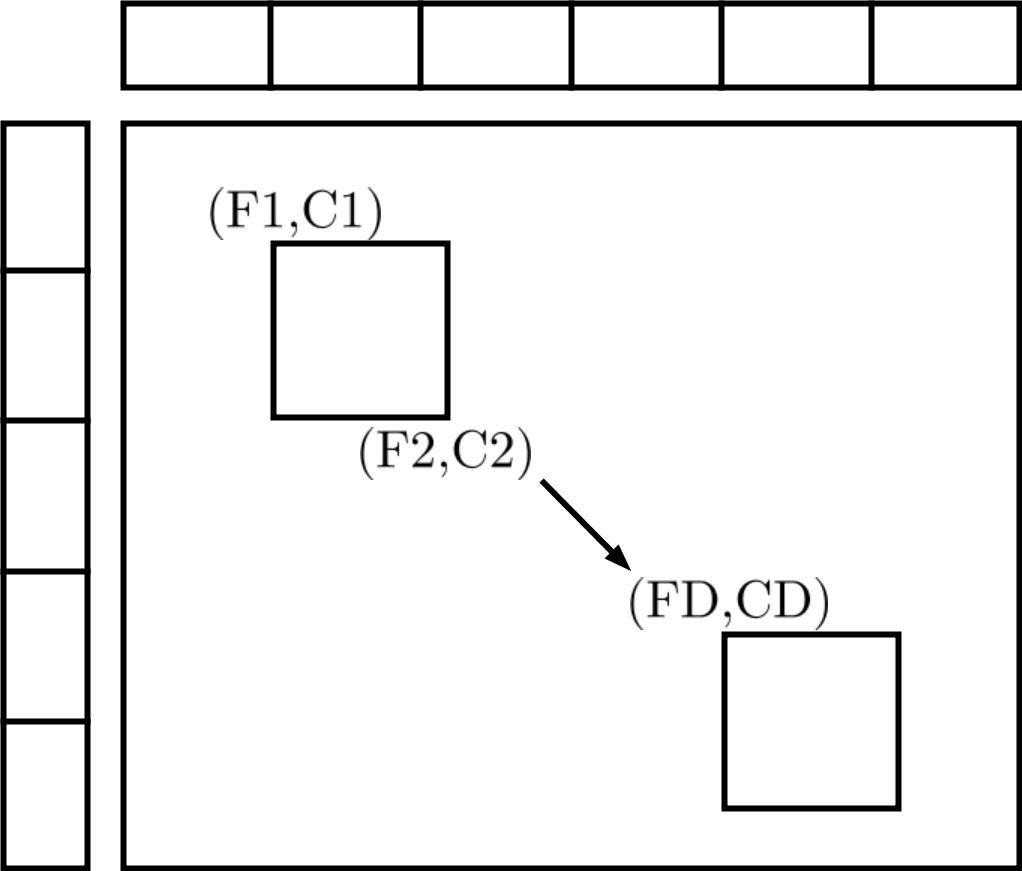
\includegraphics[scale=.2]{hojaCalculo.jpg}
\end{center}

\section{Árbol de expresiones}
\label{sec:arbol-de-expresiones}

Dada una clase ArbolExp, que representa un árbol de expresiones,
escriba un método \textbf{valor()} que de como resultado el valor de
la expresión representada. Puede suponer que sólo existen los
operadores de suma, resta, muliplicación y división. También se supone
que todos los operandos son constantes, es decir no hay variables. No
debe utilizar ninguna estructura de datos adicional. Suponga que sólo
existen las siguientes variables en cada clase:
\begin{lstlisting}[style=miEstilo, numbers=none]
class ArbolExp{
public:
   ...
   int valor();
   ...
private:
   NodoExp *raiz;
   ...
};

class NodoExp{
   ...
   void *valor;//constante u operador
   NodoExp *izq;
   NodoExp *der;
   ...
};
\end{lstlisting}

La solución es la siguiente:
\begin{lstlisting}[style=miEstilo, numbers=none]
  int ArbolExp::valor(){
    return valor(raiz);
  }

  int ArbolExp::valor(NodoExp* n){
    char * s;

    if(n==NULL)
      return -1;

    s=(char *) n->valor;//se asume que valor apunta a una cadena

    if(strcmp(s,"*")==0)
      return valor(n->izq)*valor(n->der);
    else if(strcmp(s,"/")==0)
      return valor(n->izq)/valor(n->der);
    else if(strcomp(s,"+")==0)
      return valor(n->izq)+valor(n->der);
    else if(strcmp(s,"-")==0)
	return valor(n->izq)-valor(n->der);
    else
      return atoi(s);
  }
\end{lstlisting}


\section{Tabla de Hash}
\label{sec:tabla-de-hash}

Explique los cuatro elementos generales de una tabla de dispersión.

\begin{description}
\item[Tabla: ] En esta se guarda los elementos del universo.
\item[Función Hash: ] También conocida como funcion de dispersión y da
  la posición en la tabla para una llave pasada como parámetro.
\item[Colisiones: ] Ocurre cuando dos llaves distintas dan posiciones
  de tabla coincidentes. Se debe adoptar alguna política de resolución
  de colisiones, como encadenamiento simple por ejemplo, para
  solucionarlo.
\item[Universo: ] Son elementos que posiblemente se añadirán en la
  tabla y no necesariamente ocupan espacio de memoria.
\end{description}


\section{Direccionamiento abierto de doble dispersión}

En una tabla de dispersión de tamaño $M=13$, con $h(llv)=llv \;mod\; M$,
$S(llv,i)=(llv \;mod\; 7\; + \;1)*i$, y utilizando direccionamiento abierto de
doble dispersión, realice la inserción de las siguientes llaves:
15,26, 29,2,18,28.

\begin{itemize}
\item Tamaño M=13
\item Función de dispersión $h(llv)=llv\; mod \;M$
\item Función de doble dispersión $S(llv,i)=(llv \;mod\; 7+1)$
\end{itemize}


\begin{figure}[H]
  \centering
  \begin{tabular}{|c|c|c|c|c|}
    \hline 
    LLave & $h(llv)$ & $h(llv)+S(llv,1)$ & $h(llv)+S(llv,2)$ &Posición final\\
    \hline
    16    & 15 mod 13=2 & No hay colisión       & No hay colisión &  2\\
    26    & 26 mod 13=0 & No hay colisión       & No hay colisión &  0\\
    29    & 19 mod 13=3 & No hay colisión       & No hay colisión &  3\\
    2     &  2 mod 13=2 & 2+(2 mod 7 + 1)*1=5   & No hay colisión &  5\\
    18    & 18 mod 13=5 & 5+(18 mod 7 + 1)*1=10 & No hay colisión &  10\\
    28    & 28 mod 13=2 & 2+(28 mod 7 + 1)*1=3  & 2+(28 mod 7 + 1)*2=4& 4\\
    \hline
  \end{tabular}
  \caption{Insertando valores}
\end{figure}


\begin{figure}[H]
  \centering
  \begin{tabular}{|c|}
    \hline
    26\\
    \hline
    \\
    \hline
    15\\
    \hline
    29\\
    \hline
    28\\
    \hline
    2\\
    \hline
    \\
    \hline
    \\
    \hline
    \\
    \hline
    \\
    \hline
    28\\
    \hline
    \\
    \hline
    \\
    \hline
  \end{tabular}
  \caption{Tabla resultante}
\end{figure}

\section{Búsqueda de texto}

Describa paso a paso, las distintas comparaciones o corrimientos, que
se realizaría al buscar el patrón ''\textbf{ABDCDE}'' en el texto
''\textbf{ABXDEEEBDEAABDE}'' usando la búsqueda de Booyer-Moore.

\section{Criptografía}

Con una técnica de criptografía pública, definimos $E(P_{pbl},T)$ como
el encriptado del texto $T$ con llave pública $P_{pbl}$ de la persona
$P$ y $E(P_{prv},T)$ como el encriptado del texto $T$ con la llave
privada $P_{prv}$ de la persona P. Tambíen definimos $D(P_{pbl},C)$
como el desencriptado del criptograma $C$ con la llave pública
$P_{pbl}$ de la persona $P$ y $D(P_{prv},C)$ como el desencriptado del
criptograma $C$ con la llave privada $P_{prv}$ de la persona $P$. Si
una persona $X$ desea enviar un mensaje a un sujeto $Y$, de modo que
$X$ esté seguro que sólo $Y$ podrá leer el mensaje y $Y$ esté seguro
que sólo $X$ pudo haber enviado el mensaje. Indique cómo $X$ deberá
encriptar el mensaje y cómo $Y$ deberá desencriptarlo pra lograr este
objetivo.

La \textbf{solución} es la siguiente: la persona $X$ encripta así:
\begin{eqnarray*}
  C_1&=& E(X_{prv},T)\\
  C_2&=&E(Y_{pbl},C_1)
\end{eqnarray*}

la persona $Y$ desencripta así:
\begin{eqnarray*}
  C_1&=& D(Y_{prv},C_2)\\
  T&=&D(X_{pbl},C_1)
\end{eqnarray*}

%%% Local Variables:
%%% mode: latex
%%% TeX-master: "tedd"
%%% End:


\end{document}

%%% Local Variables:
%%% TeX-master: t
%%% compile-command: "make clean"
%%% End:

